 \documentclass[oneside,a4paper,12pt]{book}
%\pagestyle{headings}
\frontmatter

%=============================================================================

\usepackage{amsthm}
\usepackage{xspace}
\usepackage{float}
\usepackage{ifthen}
\usepackage{amsbsy}
\usepackage{amssymb}
\usepackage{balance}
\usepackage{booktabs}
\usepackage{graphicx}
\usepackage{rotating}
\usepackage{multirow}
\usepackage{needspace}
\usepackage{microtype}
\usepackage{bold-extra}
\usepackage{geometry}
\usepackage{varioref}
\usepackage{xcolor}
\usepackage{textcomp}
\usepackage{listings}
\usepackage[normalem]{ulem} %emphasize still italic
\usepackage{ucs}

% \usepackage[utf8]{inputenc}
% \usepackage[htt]{hyphenat}
\usepackage{times}
\usepackage{url}
\usepackage{alltt}
\usepackage{amsmath}
\usepackage{xfrac}
\usepackage{subfigure}
\usepackage{appendix}
\usepackage{stmaryrd}   % for the \shortuparrow
\usepackage[utopia]{quotchap}

\usepackage{setspace}
\usepackage[numbers, sort&compress]{natbib}
\usepackage{mdwlist}        % support for better spaced lists
% allows for temporary adjustment of side margins
\usepackage{chngpage}
\usepackage[normalem]{ulem} 

% lina entered
\usepackage{indentfirst}
\usepackage[parfill]{parskip}
\usepackage[bottom]{footmisc}

\usepackage[T1]{fontenc}
\usepackage{caption}
\usepackage{booktabs}
\usepackage{siunitx}


\setlength{\parindent}{1.5em}

% constants

\newcounter{qcounter}

% commands
\newcommand{\n}{$\cdot$}
\newcommand{\y}{\checkmark}
\newcommand{\subscript}[1]{$_{\textrm{\footnotesize{#1}}}$}
\newcommand{\superscript}[1]{$^{\textrm{\footnotesize{#1}}}$}
\newcommand{\vertical}[1]{\raisebox{-4em}{\begin{sideways}{#1}\end{sideways}}}
\newcommand\tab[1][1cm]{\hspace*{#1}}

\usepackage{boxedminipage}

\newboolean{showedits}
\setboolean{showedits}{true} % toggle to show or hide edits
\ifthenelse{\boolean{showedits}}
{
       \newcommand{\ugh}[1]{\textcolor{red}{\uwave{#1}}} % please rephrase
       \newcommand{\ins}[1]{\textcolor{blue}{\uline{#1}}} % please insert
       \newcommand{\del}[1]{\textcolor{red}{\sout{#1}}} % please delete
       \newcommand{\chg}[2]{\textcolor{red}{\sout{#1}}{\ra}\textcolor{blue}{\uline{#2}}} % please change
}{
       \newcommand{\ugh}[1]{#1} % please rephrase
       \newcommand{\ins}[1]{#1} % please insert
       \newcommand{\del}[1]{} % please delete
       \newcommand{\chg}[2]{#2}
}


% ============================================================================
% Put edit comments in a really ugly standout display

\usepackage{xcolor}
\usepackage[normalem]{ulem}
\newcommand{\ra}{$\rightarrow$}
\usepackage{amssymb}

% comments \nb{label}{color}{text}
\newboolean{showcomments}
\setboolean{showcomments}{true}
%\setboolean{showcomments}{false}
\ifthenelse{\boolean{showcomments}}
{\newcommand{\nb}[3]{
  {\colorbox{#2}{\bfseries\sffamily\scriptsize\textcolor{white}{#1}}}
  {\textcolor{#2}{\sf\small$\blacktriangleright$\textit{#3}$\blacktriangleleft$}}}
    \newcommand{\version}{\emph{\scriptsize$-$Id$-$}}
%	 \newcommand{\ugh}[1]{\textcolor{red}{\uwave{#1}}} % please rephrase
%	 \newcommand{\ins}[1]{\textcolor{blue}{\uline{#1}}} % please insert
%	 \newcommand{\del}[1]{\textcolor{red}{\sout{#1}}} % please delete
%	 \newcommand{\chg}[2]{\textcolor{red}{\sout{#1}}{\ra}\textcolor{blue}{\uline{#2}}} % please change
	 \newcommand{\chk}[1]{\textcolor{ForestGreen}{#1}} % changed, please check
	}
{\newcommand{\nb}[3]{}
  \newcommand{\version}{}
  \newcommand{\chk}[1]{} % changed, please check
  }
\newcommand\nm[1]{\nb{NM}{violet}{#1}} % add more author macros here
\newcommand\lt[1]{\nb{LT}{orange}{#1}}


% ============================================================================
% Make quotes be italic
\renewenvironment{quote}
    {\list{}{\rightmargin\leftmargin}%
     \item\relax\begin{it}}
    {\end{it}\endlist}

\newcommand{\ttimes}{\ensuremath{\times}}

%=============================================================================

\newcommand{\needlines}[1]{\Needspace{#1\baselineskip}}

% source code
\usepackage{xcolor}
\usepackage{textcomp}
\usepackage{listings}
\definecolor{javared}{rgb}{0.6,0,0} % for strings
\definecolor{javagreen}{rgb}{0.25,0.5,0.35} % comments
\definecolor{javapurple}{rgb}{0.5,0,0.35} % keywords
\definecolor{javadocblue}{rgb}{0.25,0.35,0.75} % javadoc

\renewcommand{\lstlistingname}{Code}% Listing -> Algorithm
\renewcommand{\lstlistlistingname}{List of \lstlistingname s}% List of Listings -> List of Algorithms

\lstnewenvironment{Java}[1][]
{\lstset{
	language=Java,
	basicstyle=\footnotesize\ttfamily,
	keywordstyle=\color{javapurple}\bfseries,
	stringstyle=\color{javared},
	commentstyle=\color{javagreen},
	morecomment=[s][\color{javadocblue}]{/**}{*/},
	numbers=left,
	numberstyle=\tiny\color{black},
	stepnumber=1,
	numbersep=10pt,
	tabsize=4,
	showspaces=false,
	showstringspaces=false,
	breaklines=true,
	captionpos=b,
	xleftmargin=2em,
	framexleftmargin=1.5em,
	frame=single,
	#1
}}
{}


\lstnewenvironment{JVMIS}[1][]
{\lstset{
	language=JVMIS,
	basicstyle=\footnotesize\ttfamily,
	keywordstyle=\color{javagreen}\bfseries,
	stringstyle=\color{javared},
	commentstyle=\color{javagreen},
	morecomment=[s][\color{javadocblue}]{/**}{*/},
	numbers=none,
	numberstyle=\tiny\color{black},
	stepnumber=1,
	numbersep=10pt,
	tabsize=4,
	showspaces=false,
	showstringspaces=false
	breaklines=true,
	captionpos=b,
	xleftmargin=2em,
	framexleftmargin=1.5em,
	frame=single,
	#1
}}
{}


\definecolor{codegray}{gray}{0.9}
\newcommand{\code}[1]{
	\colorbox{codegray}
	{\texttt{#1}}
}

%----------------------------------------------------------------------------
% references
\newcommand{\tabref}[1]{\hyperref[{tab:#1}]{Table~\ref*{tab:#1}}}
\newcommand{\figref}[1]{\hyperref[{fig:#1}]{Figure~\ref*{fig:#1}}}
\newcommand{\secref}[1]{\hyperref[{sec:#1}]{Section~\ref*{sec:#1}}}
\newcommand{\subsecref}[1]{\hyperref[{subsec:#1}]{Subsection~\ref*{subsec:#1}}}
\newcommand{\lstref}[1]{\hyperref[{lst:#1}]{Listing~\ref*{lst:#1}}}
\newcommand{\charef}[1]{\hyperref[{ch:#1}]{Chapter~\ref*{ch:#1}}}
\newcommand{\coderef}[1]{\hyperref[{code:#1}]{Code~\ref*{code:#1}}}
\newcommand{\bytecoderef}[1]{\hyperref[{bytecode:#1}]{Bytecode~\ref*{bytecode:#1}}}
\newcommand{\algref}[1]{\hyperref[{alg:#1}]{Algorithm~\ref*{alg:#1}}}
\newcommand{\boxref}[1]{\hyperref[{box:#1}]{Box~\ref*{box:#1}}}

%----------------------------------------------------------------------------

% abbreviations
\tracingcolors 4
\setcounter{tocdepth}{3}
\setcounter{secnumdepth}{3}
\newcommand{\ie}{\emph{i.e.,}\xspace}
\newcommand{\eg}{\emph{e.g.,}\xspace}
\newcommand{\etc}{\emph{etc.}\xspace}
\newcommand{\etal}{\emph{et al.}\xspace}


\newcommand{\newevenside}{
	\ifthenelse{\isodd{\thepage}}{\newpage}{
	\newpage
        \phantom{placeholder} % doesn't appear on page
	\thispagestyle{empty} % if want no header/footer
	\newpage
	}
}

\def\stretchfactor{1}
\newcommand{\mychapter}[1]{\setstretch{1}
    \chapter{#1}\setstretch{\stretchfactor}}

%----------------------------------------------------------------------------
\newcommand{\lessSpace}{\vspace{-1em}}
\DeclareGraphicsExtensions{.pdf,.png}
\graphicspath{{images/}}
\newcommand{\fig}[4]{
	\begin{figure}[#1]
		\centering
		\includegraphics[width=#2\textwidth]{#3}
		\lessSpace
		\caption{\label{fig:#3}#4}
	\end{figure}}

% ===========================================================================

%:CONFIGURE THIS

\newcommand{\thesistitle}{Where does this null come from ?}
\newcommand{\thesisauthor}{Lina Tran}
\newcommand{\thesisauthorOrigin}{Biel/Bienne BE, Switzerland}
\newcommand{\thesisleiter}{Prof.\ Dr.\ Oscar Nierstrasz}
\newcommand{\thesisasst}{	\begin{center}
														Research assistant Nevena Milojkovi\'{c}\\
														Research assistant Boris Spasojevi\'{c}
													\end{center}}
\newcommand{\thesisurl}{http://scg.unibe.ch/}
\newcommand{\thesissubtitle}{An Approach to show the exact location where a value was referenced to null}
\newcommand{\thesisdate}{31. July 2016}

% ===========================================================================

\usepackage[ colorlinks=true, urlcolor=black, linkcolor=black,
			citecolor=black, bookmarksnumbered=true, bookmarks=true,
			plainpages=false,
			pdftitle={\thesistitle}, pdfauthor={\thesisauthor},
			pdfsubject={\thesissubtitle}, pdfpagelabels]{hyperref}

\newcommand{\hrref}[2]{\hyperref}
% ===========================================================================
% ===========================================================================


% D O C U M E N T
% % % % % % % % % % % % % % % % % % % % % % % % % % % % % % % % % %
\begin{document}

% T I T L E
% % % % % % % % % % % % % % % % % % % % % % % % % % % % % % % % % %
\begin{titlepage}  
  \begin{center}  
  
  \begin{figure}[t]  
  \vspace*{-2cm}        % to move header logo at the top 
  \center{
\includegraphics[scale=0.5]{logos/UNI_Bern.png}}
  \vspace{1in}     
  \end{figure}

    \thispagestyle{empty}
    
    {\bfseries\Huge \thesistitle \par
    \Large \vspace{0.1in} \thesissubtitle \par}

    \vspace{0.3in} 
    \LARGE{\textbf{Bachelor Thesis} \\}
    \vspace{0.4in}

    {\Large \thesisauthor \par from \par \thesisauthorOrigin}
    
    \vspace{0.3in}
    {\Large Faculty of Science \\
            University of Bern \par}
    \vspace{0.3in}
    {\Large \thesisdate \par}
    \vspace{0.3in}
    %Leiter der Arbeit: \par
   {\Large \thesisleiter} \par
      {\Large \thesisasst} \par
   \vspace{0.1in}
    {\Large Software Composition Group \par Institute for Computer Science \par University of Bern, Switzerland \par}
  

  %\vspace{0.5in}
 
 

  \end{center}

\end{titlepage}


% A B S T R A C T
% % % % % % % % % % % % % % % % % % % % % % % % % % % % % % % % % %
\chapter*{\centering Abstract}
\begin{quotation}
\noindent
A previous study found out that \npe are the most frequently occurring and difficult to debug exceptions in Java projects. They are difficult to debug because the developer is only provided with a stack trace to where the exception was thrown. This only gives insight into the effect of the fault but not into its cause.

The aim of the project is to provide the developer with an additional stack trace of where the variable that caused the \npe was actually set to null. We attempt to achieve this goal by instrumenting java source code striving for a minimal execution overhead.

By tracking the null assignments through static analysis and instrumentation of the bytecode we can achieve a more efficient debugging process after an occurrence of a \npe.
\end{quotation}
\clearpage


% C O N T E N T S
% % % % % % % % % % % % % % % % % % % % % % % % % % % % % % % % % % % % % % % %
\tableofcontents

\mainmatter
%%%%%%%%%%%%%%%%%%%%%%%%%%%%%%%%%%
%%%% NEW CHAPTER %%%%%%%%%%%%%%%%%%%%%
%%%%%%%%%%%%%%%%%%%%%%%%%%%%%%%%%%
\chapter{Introduction}
\label{ch:introduction}
Nowadays, practically all Java developers are at some point confronted with \npes in both big and small Java projects. Previous research has found that 35\% of conditional checks in Java projects are null checks~\cite{Osma15a}. This reduces the readability of source code and has a negative impact on performance~\cite{Osma15a}. It is also considered the number one error Java programmers make\footnote{\url{http://www.javacoffeebreak.com/articles/toptenerrors.html}}.

\Npe is a commonly occurring \rte in object-oriented languages. In most OOP languages  there is a special value called \textit{null} that is assigned to pointers (or references) in order to indicate that the pointer does not point to an object. A \npe are caused by invoking a method or accessing a field through a null value reference.

To better understand occurrences of \npes we present two different situations in which a \npe can be thrown.

\begin{Java}[caption={\Npe example (I).}, label={code:npeExampleMethodReceiver}]
public void drop(...) {
	..
	try {
		..
		DNDFigures (@\textbf{ff}@) = DNDHelper.processReceivedData(...);
		..
		Point theO = (@\textbf{ff}@).getOrigin();
		..
	}
	catch (NullPointerException npe) {
		npe.printStackTrace();
		..
	}
	..
}
\end{Java}

Assume that in the example shown in \coderef{npeExampleMethodReceiver}\footnote{\label{codeTaken1}Code snippet is a modified version of code taken from JHotDraw project: \url{http://www.jhotdraw.org/}} the variable \code{ff} at line 5 is assigned the null value from the return value of the function \code{DNDHelper.processReceivedData()}. This means that the same variable \code{ff} is \code{null} at line 9 and when a method is called on this object a \npe is thrown. Because the \npe occurred in the \code{try\{\}} block the following \code{catch\{\}} block will handle the exception by printing the stack trace. The stack trace takes the developer to line 7 where the exception was caused but not to the real culprit which is the assignment at line 5. 

\begin{Java}[caption={\Npe example (II).}, label={code:npeExampleFieldAccess}]
public class DrawApplication {
	..
	private IconkitManager (@\textbf{fManager}@);

	protected void open(...) {
		..
		createIconkit();
		..
		setTool(...);
		..
	}

	protected Iconkit createIconkit() {
		(@\textbf{fManager}@) = getIconkitManager();
		..
	}
	
	protected getIconkitManager() {
		return null;
	}

	public void setTool(...) {
		..
		(@\textbf{fManager}@).getComponent();
		..
	}
	..
}
\end{Java}

A more complicated way a \npe can be triggered is when it involves variables with larger scopes such as class members. \coderef{npeExampleFieldAccess}\textsuperscript{\ref{codeTaken1}} shows such a situation.

The \code{open()} method calls the methods \code{createIconkit()} at line 7 and \code{setTool()} at line 9. The former will initialize the field \code{fManager} (line 3) and the latter will cause the \npe.

By calling \code{createIconkit()} the field is assigned \textbf{null} by calling \code{getIconkitManager()} at line 14 which just returns the \textbf{null} value at line 19.

In the method \code{setTool()} (line 22) the \npe is finally caused by the attempt to access the field at line 24. The resulting \npe stack trace is shown in \boxref{stackTrace}:

\begin{figure}[H]
\renewcommand\figurename{Box}
	\begin{boxedminipage}{\textwidth}
		\color{cadmiumred}
		Exception in thread "main" \textcolor{blue}{java.lang.NullPointerException}\newline
		\tab at org.jhotdraw.application.DrawApplication.setTool(\textcolor{blue}{DrawApplication.java:24})\newline
		\tab at org.jhotdraw.application.DrawApplication.open(\textcolor{blue}{DrawApplication.java:9})\newline
	 \tab ...
	\end{boxedminipage}
	\caption{Stack trace of a \npe.}
	\label{box:stackTrace}
\end{figure}

In \boxref{stackTrace} we can see that the stack trace does not track to the location where the variable is assigned the null value. We call this location the root of an exception. That means the Java developer has to debug his/her way to the exception root.

At this point we introduce our project named \textit{\textbf{NullSpy}} which supports the developers in situations discussed previously. The main goal of NullSpy is to take a step towards minimizing the time spent debugging \npes. The intention behind NullSpy is to, once an unhandled \npe has occurred, present the developers the exact location of the null assignment next to the ordinary stack trace as shown in \boxref{stackTrace2}.

\begin{figure}[H]
\renewcommand\figurename{Box}
	\begin{boxedminipage}{\textwidth}
		\color{cadmiumred}
		Field this.fManager at line 14 is null: (\textcolor{blue}{DrawApplication.java: 14})\\
		Exception in thread "main" \textcolor{blue}{java.lang.NullPointerException}\\
		\tab at org.jhotdraw.application.DrawApplication.setTool(\textcolor{blue}{DrawApplication.java:24})\\
		\tab at org.jhotdraw.application.DrawApplication.open(\textcolor{blue}{DrawApplication.java:9})\\
	 \tab ...
	\end{boxedminipage}
	\caption{Stack trace of a \npe with NullSpy.}
	\label{box:stackTrace2}
\end{figure}

In this thesis we explain how the goal mentioned above is achieved and we also discuss the challenges, the limitations and performance impact of the approach.

\chapter {Technical Background}
\label{ch:technicalBackground}

This chapter provides a short overview of technologies used in the implementation of NullSpy.

\section{Bytecode}
\label{sec:bytecode}
The backbone of NullSpy is analysis and modification of Java bytecode. Java bytecode is an abstract machine language that the stack-based Java virutal machine (JVM) can understand and execute. A JVM keeps an operand stack which is modified every time the JVM executes an instruction. The instruction is represented by an opcode which also has a string representation.

Since bytecode plays an important role in our project, we will describe the Java bytecode and explain some terms we use often in this thesis. We start with an easy \textit{HelloWorld} source code example (\coderef{helloWorld}) and its bytecode (\bytecoderef{helloWorld}). 

\begin{Java}[caption={Hello World example.}, label={code:helloWorld}][H]
public class HelloWorld {
	private String hello = "Hello World!";

	public void say() {
		String result = hello;
		System.out.println(result);
	}
}
\end{Java}

\renewcommand\lstlistingname{Bytecode}
\begin{JVMIS}[numbers=left, caption={Bytecode of \coderef{helloWorld}.}, label={bytecode:helloWorld}, breaklines=true][H]
// Compiled from HelloWorld.java (version 1.8 : 52.0, super bit)
public class HelloWorld {
  
  // Field descriptor #6 Ljava/lang/String;
  private java.lang.String hello;
  
  // Method descriptor #8 ()V
  // Stack: 2, Locals: 1
  public HelloWorld();
     0  aload_0 [this]
     1  invokespecial java.lang.Object() [10]
     4  aload_0 [this]
     5  ldc <String "Hello World!"> [12]
     7  putfield HelloWorld.hello : java.lang.String [14]
    10  return
      Line numbers:
        [pc: 0, line: 1]
        [pc: 4, line: 2]
        [pc: 10, line: 1]
      Local variable table:
        [pc: 0, pc: 11] local: this index: 0 type: HelloWorld
  
  // Method descriptor #8 ()V
  // Stack: 2, Locals: 2
  public void say();
     0  aload_0 [this]
     1  getfield HelloWorld.hello : java.lang.String [14]
     4  astore_1 [result]
     5  getstatic java.lang.System.out : java.io.PrintStream [21]
     8  aload_1 [result]
     9  invokevirtual java.io.PrintStream.println(java.lang.String) : void [27]
    12  return
      Line numbers:
        [pc: 0, line: 5]
        [pc: 5, line: 6]
        [pc: 12, line: 7]
      Local variable table:
        [pc: 0, pc: 13] local: this index: 0 type: HelloWorld
        [pc: 5, pc: 13] local: result index: 1 type: java.lang.String
}
\end{JVMIS}

We are going to look only at the bytecode of method \code{say()} which is represented by the lines 25-39 in \bytecoderef{helloWorld}. The green words in \bytecoderef{helloWorld} are called Java bytecode instructions. We will also use the term \textit{opcode} referring to individual instructions. Multiple opcode instructions are referred to as bytecode.

On the left-side of these instructions we see the \textit{program counter} (pc) which is a processor register that contains the address (location) of the instruction being executed at the current time. It is also called instruction pointer. We use these pcs also as an index in the bytecode. The instructions from pc 0 to pc 4 (lines 26-28) in \bytecoderef{helloWorld} represents the source code at line 5 in \coderef{helloWorld}. Therefore we use the term \textit{pc-interval} to describe an instruction-set that represents \eg a method invocation, an assignment \etc. This term will play an important role further in the thesis. We use the syntax ``<,>'' to represent the pc-interval. For the example just mentioned before the pc-interval <0,4> represents the source code at line 5 in \coderef{helloWorld}. The first number indicates where the pc-interval starts and the latter one where it ends, both included.

Going back to the example shown in \bytecoderef{helloWorld}, we can see on the right-side the name and type of variables, or in case of an invocation the behavior/method name and the parameters it takes \etc. In \secref{lowLevelOverview} we will see how this information is used.

Underneath the instructions from line 33-36 in \bytecoderef{helloWorld} we find the \textit{line number table}\footnote{In the jargon of Javasist, this is also called the line number attribute.}. It maps the pc to the source code line. The numbers at the end of the lines in \boxref{stackTrace} indicate the lines of code that caused the \npe. The information the \textit{line number table} holds is used to recover where the null was assigned. 

The bytecode of each behavior also holds a local variable table (\eg \bytecoderef{helloWorld} line 37-39) which is an array of local variables. All the parameters of a method and the value of the local variables are stored in this table. Parameters are stored first, beginning at index/slot 0 . But the local variable table of a constructor or an instance method stores the \textit{``hidden this''} reference first, which is used to access the instance data of the object, then the parameters and so on. In \figref{localVarArray}\footnote{Figure taken from \url{http://www.ibm.com/developerworks/library/it-haggar_bytecode/}} we see how a local variable is stored in the local variable table.

\begin{figure}[H]
\centering
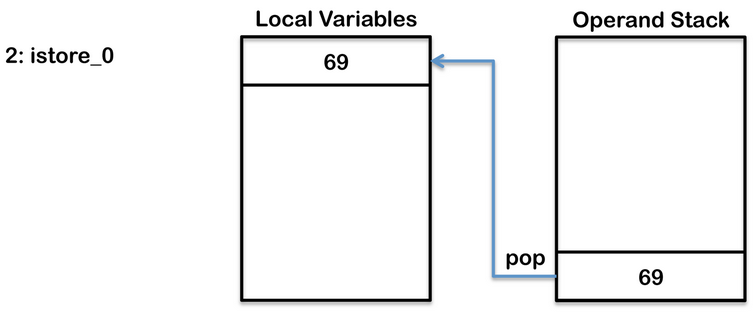
\includegraphics[width=0.8\linewidth]{localVarArray}
\caption{Local variable table/array\protect.}
  \label{fig:localVarArray}
\end{figure}

Local variables do have a limited lifespan, the square bracket of the local variable table represents the lifespan. The closing bracket \code{\}} of the block, where the local variable is created, indicates its ending.  As soon as the lifespan of one ends, the slot can be reused by the next instantiated local variable. This is why we can find local variable tables that contain multiple entries with the same local variable slot, see \bytecoderef{localVarTableDuplicatedSlot1}.


\begin{JVMIS}[numbers=left, caption={Local variable table entries with same slot 2 (line 4\&7).}, label={bytecode:localVarTableDuplicatedSlot1}, breaklines=true]
Local variable table:
 [pc: 0, pc: 95] local: this index: 0 type: org.jhotdraw.samples.javadraw.JavaDrawViewer
 [pc: 0, pc: 95] local: filename index: 1 type: java.lang.String
 [pc: 13, pc: 40] local: url index: 2 type: java.net.URL
 [pc: 18, pc: 40] local: stream index: 3 type: java.io.InputStream
 [pc: 28, pc: 40] local: reader index: 4 type: org.jhotdraw.util.StorableInput
 [pc: 44, pc: 94] local: e index: 2 type: java.io.IOException
\end{JVMIS}

\section{Javassist}
\label{sec:javassist}
\textit{Javassist} or \textit{Java Programming Assistant}\footnote{\url{http://jboss-javassist.github.io/javassist/}}~\cite{Chib00}~\cite{Chib03}, a subproject of Jboss, is a library which enables manipulation of the Java bytecode. Since 1999 it is used as an engineering toolkit in a broad domain, and is still being extended by Shigeru Chiba. It enables developers to manipulate Java bytecode in a simplified way. Examples of this manipulation include defining a new class at runtime or modifying a class file when it is loaded by the JVM. All manipulations are performed at load-time through a provided class loader. A tutorial for using Javassist\footnote{\url{http://jboss-javassist.github.io/javassist/tutorial/tutorial.html}} is available online and was used as a starting point for this work.

Unlike many other bytecode manipulation libraries, Javassist offers two levels of API: \textbf{source}-level and \textbf{bytecode}-level. Using the source-level API, the user can edit a class file without any familiarity with the specifications of the Java bytecode. Knowledge of the Java language is enough since the API is designed only with the vocabulary of Java. On this level the programmer has to write Java source code and Javassist compiles it automatically. The bytecode level allows the user to modify classes by modifying the bytecode directly.

%\begin{figure}[H]
%\centering
%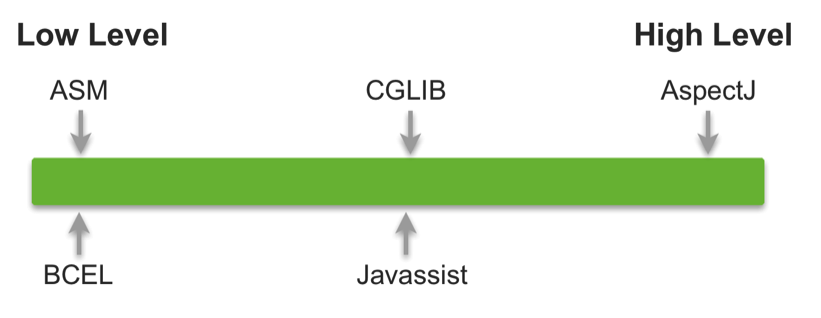
\includegraphics[width=0.8\linewidth]{javassistLevel}
%\caption{Bytecode modification levels.}
  %\label{fig:bytecodeModificationLevels}
%\end{figure}

%In \figref{bytecodeModificationLevels}\footnote{Figure taken from \href{https://blog.newrelic.com/2014/09/29/diving-bytecode-manipulation-creating-audit-log-asm-javassist/}{blog.newrelic.com}.} the term \textit{``Low Level''} is used for \textit{bytecode}-level and \textit{``High Level''} for \textit{source}-level. Using the libraries \textit{ASM} and \textit{BCEL} \brs{links or refs to these libs}the user has to construct bytecode itself and is not able to only write simple source code to modify a class file. The library \textit{AspectJ} on the other hand only allows the user to write source code which is than translated into bytecode. This way of course the user is limited by the functionality of the library \textit{AspectJ}. \textit{Javassist}\brs{not consistent, sometimes textit sometimes not. I don't see why it should be textit, I receomend droping it} and \textit{CGLIB} provide the user the choice of whether to work on \textit{bytecode}- or \textit{source}-level, or even on both. \brs{this whole story about ``levels'' is important because...}\lt{figure shows that javassist can use both apis.. take out?}

At this point, let us look at the small example shown in \coderef{javassistExample}\footnote{Example taken from Javassist tutorial.} of how the bytecode manipulation with javasist works. We go through the example line by line.

\renewcommand\lstlistingname{Code}
\begin{Java}[caption={Javassist example.}, label={code:javassistExample}][H]
ClassPool pool = ClassPool.getDefault();
CtClass cc = pool.get("test.Rectangle");
cc.setSuperclass(pool.get("test.Point"));
cc.writeFile();
\end{Java}

\begin{enumerate}
	\item First a \textit{ClassPool} object that controls bytecode modification is obtained. With the \textit{ClassPool} object a class file (``.class'') can be read on demand for constructing a \textit{CtClass} object.

	\item The class \textit{CtClass} (compile-time class) represents the class file. This means that all manipulations are performed on the \textit{CtClass} object. We obtain a reference to the \textit{CtClass} object representing the \code{test.Rectangle} class by invoking the \code{get()} method on the \textit{ClassPool} instance.

	\item In this example the only bytecode modification done is changing the superclass of \code{test.Rectangle} to \code{test.Point}. This does not serve any purpose and is only illustrative.
	\item Once the bytecode modification is done, the method call \code{writeFile()} on the instance of \textit{CtClass} is necessary to make sure that the changes are reflected on the original class file. The method \code{writeFile()} converts the modified \textit{CtClass} object into a class file and stores it on a local disk.
\end{enumerate}

\begin{figure}[H]
\centering
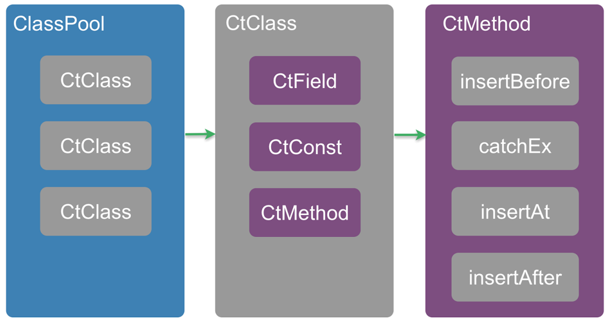
\includegraphics[width=0.8\linewidth]{javassistModules}
\caption{Javassist modules.}
  \label{fig:javassistModules}
\end{figure}

\figref{javassistModules}\footnote{Figure taken from \href{https://blog.newrelic.com/2014/09/29/diving-bytecode-manipulation-creating-audit-log-asm-javassist/}{blog.newrelic.com}.} gives an overview of how the main part of bytecode manipulation with Javassist is built up. The \textit{ClassPool} is simply a container of multiple \textit{CtClasses}. As described before \textit{CtClass} represents a class file on which modifications are done. Like typical classes, it can hold compile-time fields, constants or methods. Javassist is capable of adding or modifying classes, behaviors, fields, method invocations, local variables \etc But in our case we mainly address the manipulation of behaviors. It is possible to insert additional source code at the beginning of the method body, at the end or at a specific line. The next example shows how to add code using Javassist.

\begin{Java}[caption={Initial code.}, label={code:initialCode}][H]
public static void main(String[] args) {
	System.out.println("This is an example class.");
}
\end{Java}

\renewcommand\lstlistingname{Bytecode}
\begin{JVMIS}[caption={Initial bytecode.}, label={bytecode:initialBytecode}, breaklines=true][H]
public static void main(java.lang.String[]);
  0: getstatic     #16	// Field java/lang/System.out:Ljava/io/PrintStream;
  3: ldc           #22	// String This is an example class.
  5: invokevirtual #24	// Method java/io/PrintStream.println:(Ljava/lang/String;)V
  8: return
\end{JVMIS}

We want to add one line of code at the beginning of the \code{main()} method in \coderef{initialCode}. \bytecoderef{initialBytecode} is the corresponding bytecode of \coderef{initialCode}.

\renewcommand\lstlistingname{Code}
\begin{Java}[caption={Bytecode modifier.}, label={code:bytecodeModifier}][H]
public class BytecodeModifier {
	public static void main(String[] args) ... {
		ClassPool pool = ClassPool.getDefault();
		CtClass cc = pool.get("insertJavaCodeExample.ExampleClass");

		CtBehavior behavior = cc.getDeclaredMethod("main");
		behavior.insertBefore("System.out.println(\"This is the inserted code.\");");

		cc.writeFile();

		//...
	}
}
\end{Java}

With \coderef{bytecodeModifier} we obtain a \textit{CtClass} object \code{cc} at line 4 which represents the class to be modified. At line 7 we get the method we want to modify by adding some source code: \code{System.out.println(``This is the inserted code.'');}. Javassist takes a \textit{java.lang.String} object, compiles it automatically and adds it into the bytecode at the specified location, in our situation at the beginning of the \code{main()} method.

The source code at line 2 shown in \coderef{instrumentedCodeDecompiled} is the decompiled form of the result \ie the \code{main()} method equivalent to what we achieved with Javassist. The actual result, the modified bytecode shown in \bytecoderef{modifiedBytecode}, is the pc-interval <0,5>.

\begin{Java}[caption={Instrumented code: Decompiled with JAD (\secref{jad})}, label={code:instrumentedCodeDecompiled}][H]
public static void main(String args[]) {
	System.out.println("This is the inserted code.");
	System.out.println("This is an example class.");
}
\end{Java}

\renewcommand\lstlistingname{Bytecode}
\begin{JVMIS}[caption={Modified bytecode.}, label={bytecode:modifiedBytecode}, breaklines=true][H]
public static void main(java.lang.String[]);
  0: getstatic     #16 	// Field java/lang/System.out:Ljava/io/PrintStream;
  3: ldc           #35	// String This is the inserted code.
  5: invokevirtual #24	// Method java/io/PrintStream.println:(Ljava/lang/String;)V
  8: getstatic     #16	// Field java/lang/System.out:Ljava/io/PrintStream;
 11: ldc           #22	// String This is an example class.
 13: invokevirtual #24	// Method java/io/PrintStream.println:(Ljava/lang/String;)V
 16: return
\end{JVMIS}

\section{JAD}
\label{sec:jad}
Java Decompier (JAD)\footnote{\url{https://sourceforge.net/projects/jadclipse/}} is a decompiler and an Eclipse plugin for the programming language Java. A decompiler is a program that takes an executable file as input, and attempts to create a high level, compatible source file. If the source file is compiled again, it will produce an executable program that behaves the same way as the original one. It is often used in software reverse engineering.

The example \bytecoderef{jad} is decompiled by JAD and the result is the source code shown in \coderef{decompiledBytecode}.

\begin{JVMIS}[caption={Bytecode example.}, label={bytecode:jad}, breaklines=true]
public void itemStateChanged(java.awt.event.ItemEvent e);
  0  aload_1 [e]
  1  invokevirtual java.awt.event.ItemEvent.getStateChange() : int [23]
  4  iconst_1
  5  if_icmpne 22
  8  aload_0 [this]
  9  getfield org.jhotdraw.applet.DrawApplet$1.this$0 : org.jhotdraw.applet.DrawApplet [12]
 12  aload_1 [e]
 13  invokevirtual java.awt.event.ItemEvent.getItem() : java.lang.Object [29]
 16  checkcast java.lang.String [33]
 19  invokevirtual org.jhotdraw.applet.DrawApplet.loadDrawing(java.lang.String) : void [35]
 22  return
Line numbers:
 [pc: 0, line: 213]
 [pc: 8, line: 214]
 [pc: 22, line: 216]
Local variable table:
 [pc: 0, pc: 23] local: this index: 0 type: new org.jhotdraw.applet.DrawApplet(){}
 [pc: 0, pc: 23] local: e index: 1 type: java.awt.event.ItemEvent
\end{JVMIS}

\renewcommand\lstlistingname{Code}
\begin{Java}[caption={Decompiled bytecode.}, label={code:decompiledBytecode}]
public void itemStateChanged(ItemEvent e) {
	if(e.getStateChange() == 1)
	loadDrawing((String)e.getItem());
}
\end{Java}

JAD is in no way a dependency of NullSpy but it was a big help during the implementation phase since after running NullSpy on a project only the modified bytecode is available. The use of JAD is for the sake of debugging Nullspy; to check whether the modification by Javassist, \ie inserting source code, was successful. Another way to check the result for correctness is looking at bytecode itself but that would have taken a lot more effort and time.

\chapter{NullSpy}
As explained in \charef{introduction}, this project is about providing the user with an additional link next to the common stack trace containing the information/location of where the null is assigned to the variable that caused the \npe.

In this chapter we give an overview of how we implemented NullSpy. We will also address the challenges (\secref{challenges}) we encountered during the implementation as well as the limitations of the tool (\secref{limitations}).

\section{High Level Overview}
\label{sec:highLevelOverview}
The general approach of NullSpy is to statically analyze a project and instrument the bytecode. NullSpy is a console application which takes two arguments. The first argument to NullSpy is the path to the folder containing the compiled class files of the original project and the second one is the destination where the user wants to store the modified class files.

We provide the option to choose the destination in case the developer does not want to overwrite the original project with the modified one. This means that the updated bytecode can be stored in another location, keeping the original class files intact. Of course the original project can be replaced by the modified one too. But the developer has to think carefully about it because once replaced, the additional bytecode stays there and the execution time is slightly different than it was before. To get rid of the additional bytecode, the developer has to recompile the source code to get the original class files when needed.

\begin{figure}[H]
\centering
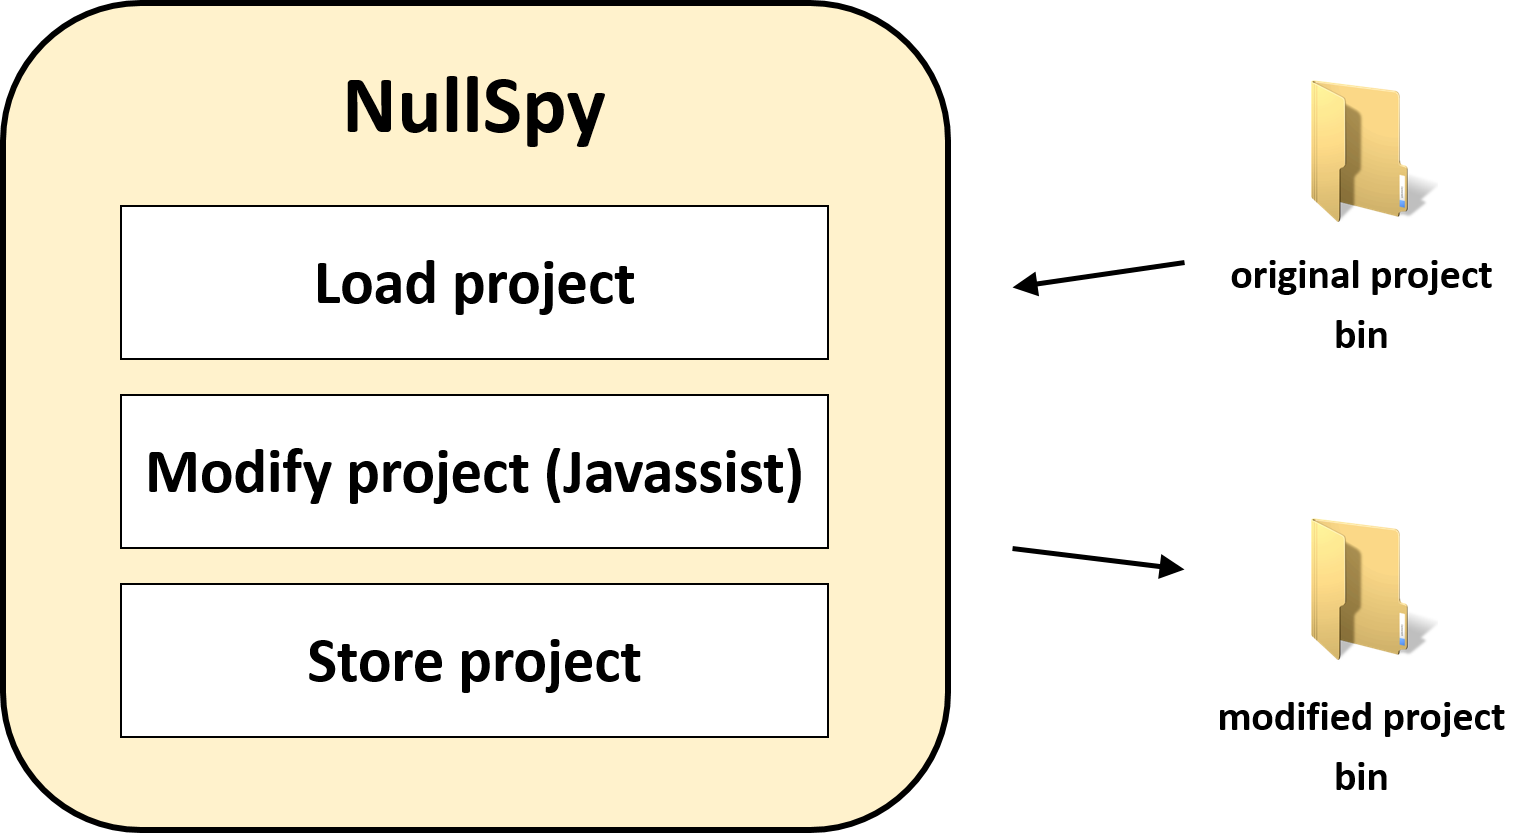
\includegraphics[width=0.8\linewidth]{highLevelOverview3}
\caption{High level overview.}
  \label{fig:highLevelOverview}
\end{figure}

NullSpy contains three basic steps which we can see in \figref{highLevelOverview}: \textit{load, modify, store}. Those three steps of NullSpy are described in \listref{abstractSteps}:

\begin{figure}[H]
\renewcommand\figurename{List}
	\begin{boxedminipage}{\textwidth}
\begin{enumerate}
\itemsep8pt
	\item Input: Load compiled class files of the project into NullSpy.
	\item Modification: The modification part deals with the bytecode instrumentation and adding modules to the project that supports the inserted code.
	\item Output: Store modified class files to the chosen output folder.
   \end{enumerate}
	\end{boxedminipage}
	\caption{NullSpy abstract steps.}
	\label{list:abstractSteps}
\end{figure}

Loading is done by traversing all the subfolders of the folder given as a parameter, and extracting all the \textit{.class} files. NullSpy modifies the class file directly when it is loaded. As soon as the modification is done, the class file is stored to the destination folder \ie the second parameter of NullSpy. 

Storing is done by recreating the structure from the source folder in the destination folder and storing the modified class files using the Javasist API. 

%\del{In secref{javassist} we store the modified class file on a local disk. This way the original class file remains intact. In our case we write the modified class file in the destination folder not only on a local disk. This way the original project can be overwritten as explained before.} \brs{what? not only on a local disk? what does that even mean}\lt{ask, javassist tutorial store on local disk, here write new file or overwrite}

\section{Low Level Overview}
\label{sec:lowLevelOverview}

In this section we will focus on the bytecode modification. \figref{modificationModules} shows that NullSpy contains three different modules in total. That means each class file of the loaded project will be run through with each of these modules. The first thing we do with the loaded class file is extracting data from its bytecode, then do the instrumentation and at the end we add the run time supporter module to the project.

\begin{figure}[H]
\centering
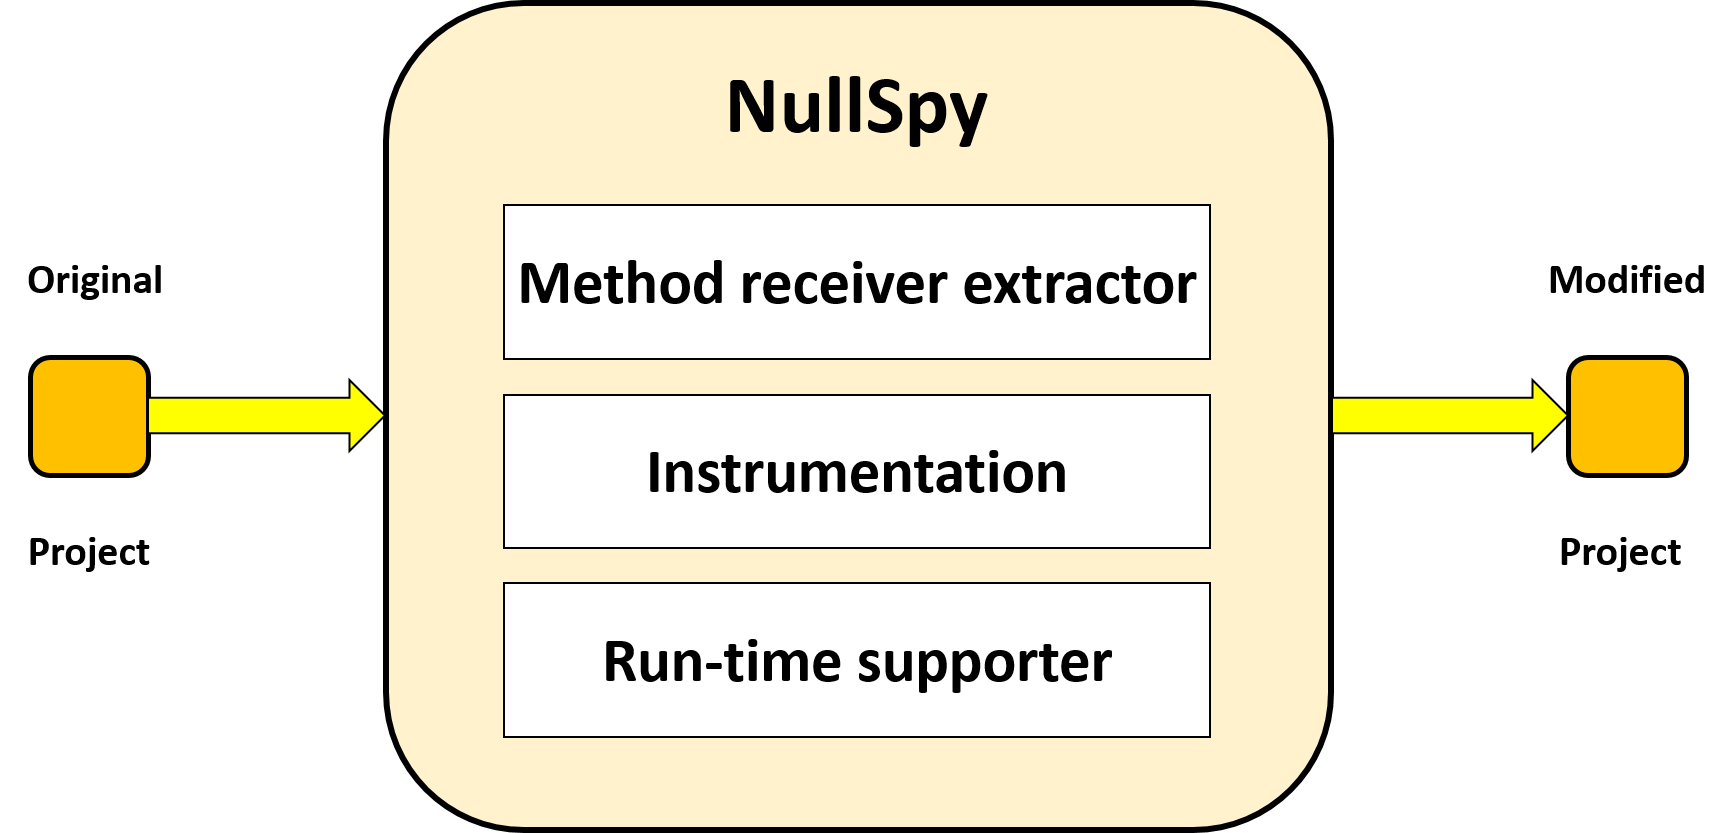
\includegraphics[width=0.8\linewidth]{lowLevelOverview}
\caption{NullSpy modification modules.}
  \label{fig:modificationModules}
\end{figure}

We will look at these modules in more detail and explain what each one does.

\subsection{Process Flow}
\label{subsec:processFlow}
In this short and rough overview of the entire process we explain the reason why we have to extract data from bytecode and what they are used for. Details are discussed in the following subsections.

From the stack trace of a \npe we can obtain three information, namely the class name, method name and the line number of where the \npe happened. But the aim of NullSpy is to reveal the location of the null assignment of the variable that caused the \npe. To achieve this goal we need to extract information from bytecode and compare them with each other to get the right location of the null assignment.

The first step in the modification part is to extract information about the \mr. We use the term \mr to refer to variables on which methods are invoked, or whose fields are accessed. The same data like obtained from the \npe stack trace and other values \eg the variable name, variable type \etc are stored.

The second step is to collect information about the null assignment. If a variable is assigned an object we gather data about the variable from the bytecode. The most important information obtained is the line number of the null assignment. Right after the assignment and the data collection NullSpy inserts some bytecode that represents a method call which is managed by the \textit{run time supporter}. This method takes those extracted information as parameters and checks whether the variable is assigned null. If it is assigned null the information about the variable is stored.

At the end of the bytecode modification part we wrap the \code{main()} method into a \textit{try-catch-block}. In the \textit{catch-block} those three information (class name, method name, line number) mentioned before are extracted from the \npe stack trace. These information are also passed on to a static method of the \textit{run time supporter}. This method compares the parameters with the stored information about the \mrs. If there is a match regarding the comparison NullSpy creates a variable identification with the information about the matched \mr. With this id another comparison is performed. This time NullSpy compares the id with the information stored about the null assignment. The result will be the stored entry about the null assignment of the variable that caused the \npe. From the entry we extract the line number of the assignment and create the additional link that reveals the location of the null assignment. This link of course is then added to the common \npe stack trace.

Finally we add the \textit{run time supporter} module to the modified project.

The way how we extract and store all those data are discussed in the following sections.

\subsection{\MR Data Collection}
\label{subsec:methodReceiver}
As mentioned in \subsecref{processFlow}, a big part of NullSpy is extracting information from bytecode. One of the item we are interested to get information about is the \mr. A small synthetic example (\coderef{methodReceiverExample}) makes is easier to understand. \Mrs in \coderef{methodReceiverExample} are the variables \code{var} at line 9, \code{field} at line 10 and \code{b.foo} at line 11.

\renewcommand\lstlistingname{Code}
\begin{Java}[caption={\Mr example.}, label={code:methodReceiverExample}]
public class A {

	private Object (@\textbf{field}@) = new Object();
	private Object b = new B();
	
	public static void main() {
		Object (@\textbf{var}@) = new Object();
		
		(@\textbf{var}@).toString();	// variable on which method is invoked
		(@\textbf{field}@).toString();	// field access
		(@\textbf{b.foo}@).toString(); // field access
	}
}

public class B {
	public Object foo = new Object();
	..
}
\end{Java}

We use the library Javassist to extract data from bytecode. Unfortunately, Javassist does not provide the functionality to directly get information about the \mr. The exact information we need is listed in \listref{methodReceiverInfo} and it is stored in an external \textit{csv} file due to overhead minimization.

\begin{figure}[H]
\renewcommand\figurename{List}
	\begin{boxedminipage}{\textwidth}
		\begin{itemize}
		\itemsep8pt
    \item counter (\mrs are counted)
		\item lineNumber
		\item variableID (whether it is a local variable or a field)
		\item variableType
		\item isVariableStatic
		\item classWhereVariableIsAccessed
		\item behavior (method)
		\item behaviorSignature
		\item localVariableAttributIndex (if variable is a local variable, else ``empty string'')
		\item fieldDeclaringClassName (if variable is a field, else ``empty string'')
   \end{itemize}
	\end{boxedminipage}
	\caption{\Mr information.}
	\label{list:methodReceiverInfo}
\end{figure}

This is why we implemented our own algorithm to get the \mrs. We need the exact pc-interval of the \mr to extract the right data from bytecode. As we discuss the steps of the algorithm we will be showing the result of each step when applied to the example source code and bytecode shown in \coderef{methodReceiverAlgDemoCode} and \bytecoderef{methodReceiverAlgDemoBytecode}. The algorithm contains following steps:

\textbf{Finding the invocation bytecode}\\
While iterating through the bytecode NullSpy looks for the opcodes which matches the regex \textit{``invoke.*''}. Each of these opcodes represents one method invocation for which we are trying to find the \mr. We call the pc of the invocation the end-pc. In our example, the end-pc is 155, since we are interested in the receiver of the \code{add} method.

\textbf{Finding the start-pc}\\
We locate the pc at which the bytecode for source code line of the invocation begins. We call this the start-pc. This is done using the line number table mentioned in \secref{bytecode}. This table is omitted from our example for simplicity and the start-pc is 144.

\textbf{Defining the outermost pc-interval}\\
We define the outermost pc-interval as the interval starting with the start-pc and ending with the end-pc. We know that the \mr is located in this interval. In our example, this is <144,155>.

\textbf{Getting the number of parameters for the method}\\
Javassist offers the functionality to count the number of parameters a method invocation has by analyzing the method signature. The signature is a \textit{String} that contains the parameter and the return type of the method call. Our example method takes 2 parameters.

\textbf{Extracting candidate \mr pc-intervals}\\
The outermost interval <144,155> could contain other invocations, which could have \mrs of their own. This is visible in our example, where the \code{getDesktop} invocation (pc 146) is embedded in our outermost interval. For this reason, we explored all possible bytecode combinations of \mrs and developed a system for identifying such embedded call sights. More about this system can be found in the appendix (\ref{cha:bytecodeCombinations}). This system allows us to split the outermost pc-interval into candidate \mr pc-intervals. In our example, the outermost pc-interval is divided into \{<144,144>,<145,149>,<152,152>\}.

\textbf{Finding the actual \mr}\\
Since the candidate pc-intervals end with the arguments of the method, and we know that the method expects $N$ arguments, we can ignore the last $N$ candidate pc-intervals. The one before them is the actual \mr pc-interval. In other words, the $N$-th to last candidate is the actual \mr pc-interval. In our example, since the method takes 2 arguments, the actual \mr pc-interval is <144,144>.

\renewcommand\lstlistingname{Code}
\begin{Java}[caption={Code snippet to demonstrate \algref{methodReceiverAlg}.}, label={code:methodReceiverAlgDemoCode}]
protected void open(final DrawingView newDrawingView) {
	//...
	activePanel.add((Component) getDesktop(), BorderLayout.CENTER);
	//...
}
\end{Java}

\renewcommand\lstlistingname{Bytecode}
\begin{JVMIS}[caption={Bytecode of \coderef{methodReceiverAlgDemoCode}.}, label={bytecode:methodReceiverAlgDemoBytecode}, breaklines=true]
protected void open(org.jhotdraw.framework.DrawingView newDrawingView);
 ...
 144  aload_3 [activePanel]
 145  aload_0 [this]
 146  invokevirtual org.jhotdraw.application.DrawApplication.getDesktop() : org.jhotdraw.contrib.Desktop [271]
 149  checkcast java.awt.Component [274]
 152  ldc_w <String "Center"> [276]
 155  invokevirtual javax.swing.JPanel.add(java.awt.Component, java.lang.Object) : void [254]
 ...
\end{JVMIS}

We had troubles getting the right outermost pc-interval of the \mr. By only statically analyzing the bytecode it is unapparent where exactly the \mr is situated in bytecode. More about the challenges we encountered can be found in \subsecref{methodReceiverDifficulties}.

Statically analyzing bytecode for \mr means looking for certain opcodes which matches the regex (Regular expression) \textit{``invoke.*''}. There are exactly five such bytecode instructions: \textit{invokedynamic}, \textit{invokeinterface}, \textit{invokespecial}, \textit{invokestatic}, \textit{invokevirtual}. The invocation opcode \textit{invokedynamic} facilitates the dynamicly-typed languages\footnote{Language whose type checking is performed at runtime.} through dynamic method invocation. In our case it can be ignored because NullSpy only supports Java, a \textit{staticlly-typed} language\footnote{Language whose type checking is performed at compile time.}.

In case of the simple stand-alone \textit{invokestatic} instruction we do have a \mr but it can be ignored because static method invocations are called on classes which can never be null. Because of this, NullSpy ignores the instruction \textit{invokestatic}. But if the static method call is a parameter of another method call, NullSpy still treats it as a \mr candidate.

As soon as we have the \mr pc-interval we can extract information about the \mr from the bytecode. The use of the Javassist API allows us to obtain the information about the \mr listed in \listref{methodReceiverInfo}.

\subsection{Variable Data Collection}
\label{subsec:variable}
In the section before we were looking for instructions which matches the regex \textit{``invoke.*''} to detect \mrs in bytecode. This time we are looking for the regexs \textit{``astore.*''} and \textit{``put.*''}. The former refers to local variable assignments and the latter to field assignments. Unlike the information collection of the \mr, the data about the variables are stored in a HashMap.

In the next two subsections we will look at how the information about the assigned variables is extracted. Due to different variable types and the limitation of Javassist, the ways of gathering information about the local variables and fields are performed differently.

\subsubsection{Local Variable}
\label{subsubsec:localVariable}
Unfortunately, Javassist does not provide any support for gaining information about local variables. This is why we have to understand how the bytecode is constructed concerning the local variables. In \secref{bytecode} we introduced the parts of the bytecode that are important for our project NullSpy. 

%\begin{figure}[H]
%\centering
%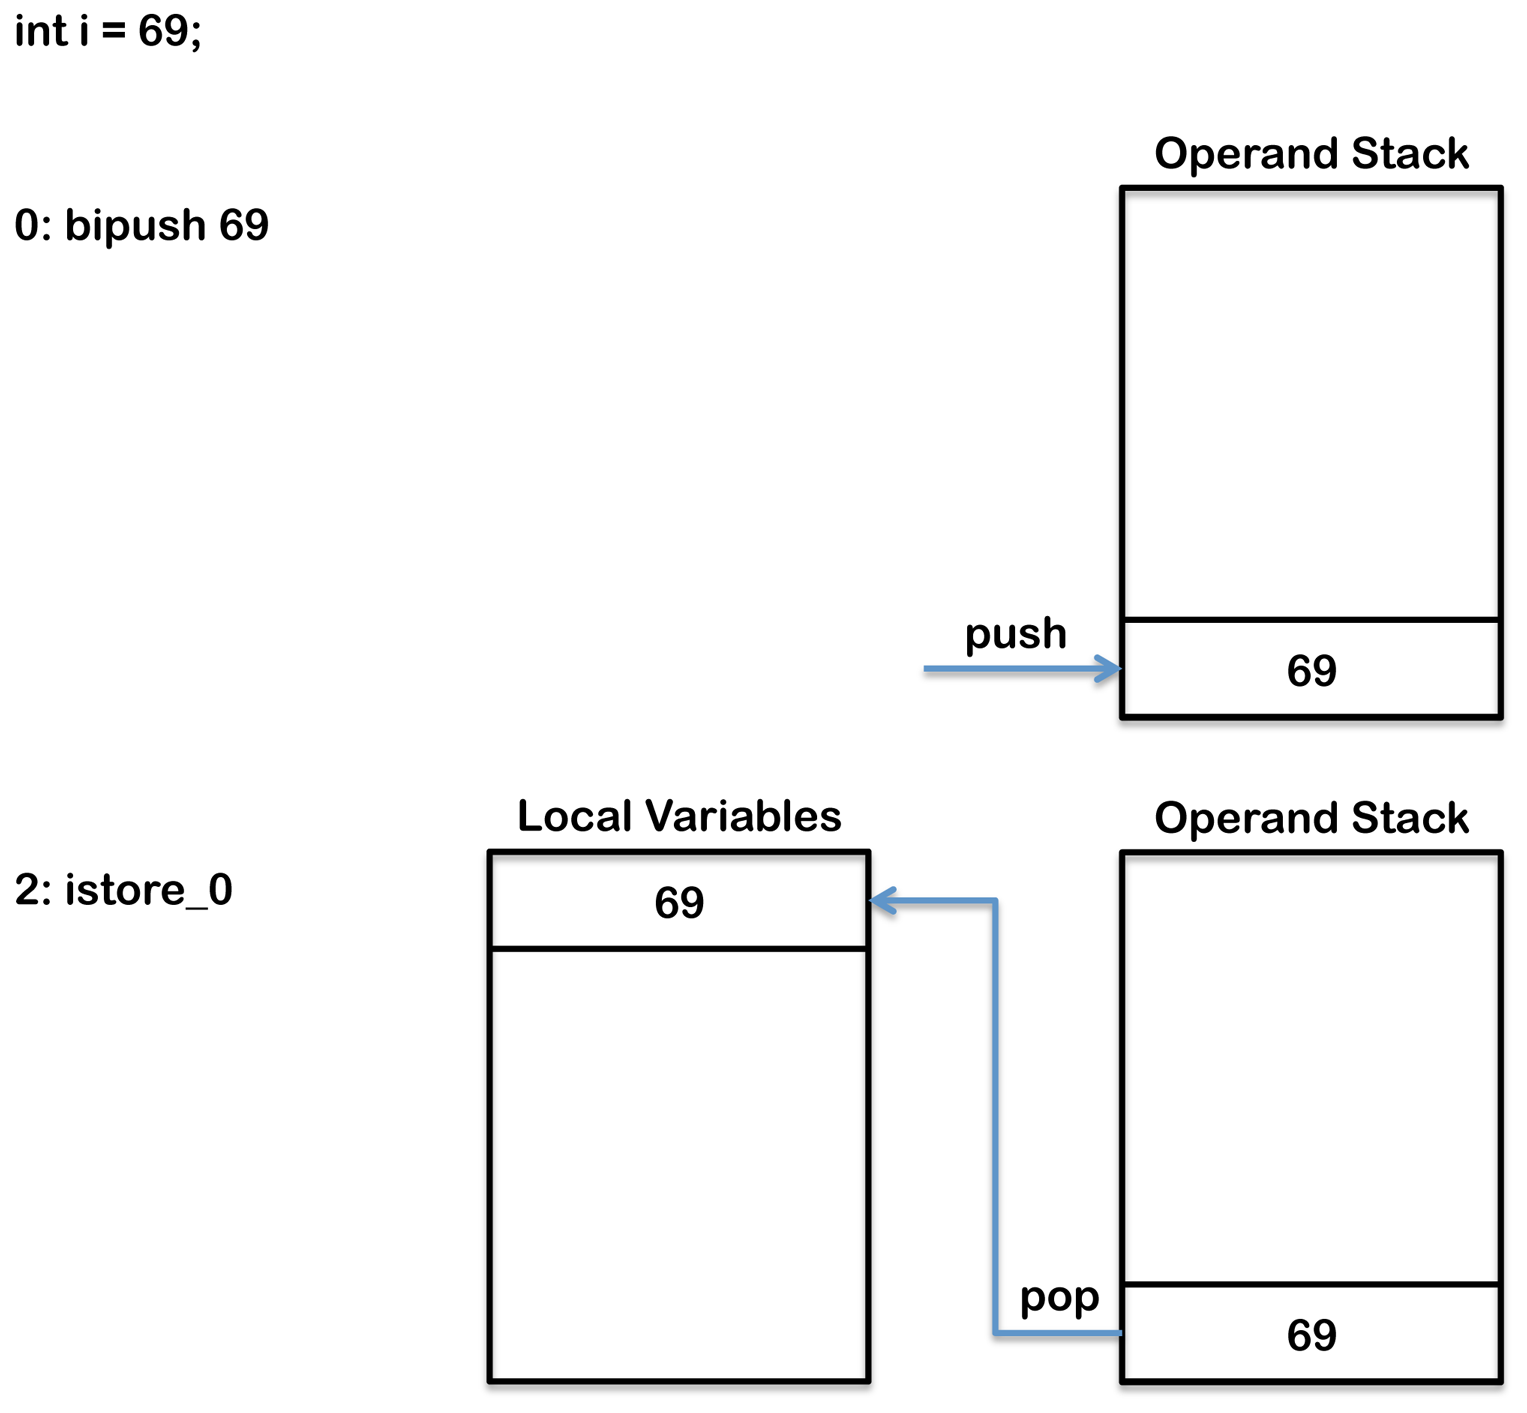
\includegraphics[width=0.8\linewidth]{localVarCreationBytecode}
%\caption{Local variable creation\protect.}
  %\label{fig:localVarCreationBytecode}
%\end{figure}

%If a local variable is created, the value assigned to it is pushed onto the operand stack as we can see in \figref{localVarCreationBytecode}\footnote{Figure taken from \href{http://blog.jamesdbloom.com/JavaCodeToByteCode_PartOne.html}{blog.jamesdbloom.com}.}. With the bytecode instruction \textit{``astore.*''} the local variable is popped from the operand stack and stored into a local variable array slot. In which slot it is stored can be extracted from the instruction. Opcodes for storing local variables are composed of one, or in some cases two bytes. There are reserved instructions for the first four created local variables. These instructions are index-linked from 0 to 3 and each of them contains one byte (astore\_0, astore\_1, astore\_2, astore\_3). If there is no slot number visible in the instruction, it indicates that the slot number is stored in the second byte from where it can be extracted.\brs{no idea what this paragraph is about}

%With this short introduction understanding the local variable table should be easier. Each method of a class file contains a local variable table (see \bytecoderef{localVarTable}) with which many information can be read out, \ie the lifespan of a local variable, what it is called, in which slot it is stored and what type it has.

%\renewcommand\lstlistingname{Bytecode}
%\begin{JVMIS}[caption={Local variable table.}, label={bytecode:localVarTable}, breaklines=true]
%Local variable table:
 %[pc: 0, pc: 31] local: this index: 0 type: org.jhotdraw.samples.javadraw.JavaDrawApp
 %[pc: 0, pc: 31] local: newDrawing index: 1 type: org.jhotdraw.framework.Drawing
 %[pc: 5, pc: 31] local: d index: 2 type: java.awt.Dimension
 %[pc: 22, pc: 31] local: newDrawingView index: 3 type: org.jhotdraw.framework.DrawingView
%\end{JVMIS}

We have to pay attention to get the right local variable every time we bump into one while iterating through bytecode. Every time we hit upon the opcode \textit{``astore.*''} we could only get its slot and the pc where it is situated in the bytecode sequence. A local variable has a limited lifespan. The lifespan of a local variable is important because multiple entries can have the same local variable slot (already described in \secref{bytecode}).

\begin{JVMIS}[numbers=left, caption={Local variable table entries with same slot 2 (line 4\&7).}, label={bytecode:localVarTableDuplicatedSlot}, breaklines=true]
Local variable table:
 [pc: 0, pc: 95] local: this index: 0 type: org.jhotdraw.samples.javadraw.JavaDrawViewer
 [pc: 0, pc: 95] local: filename index: 1 type: java.lang.String
 [pc: 13, pc: 40] local: url index: 2 type: java.net.URL
 [pc: 18, pc: 40] local: stream index: 3 type: java.io.InputStream
 [pc: 28, pc: 40] local: reader index: 4 type: org.jhotdraw.util.StorableInput
 [pc: 44, pc: 94] local: e index: 2 type: java.io.IOException
\end{JVMIS}

Iterating through the bytecode and finding the opcode \textit{``astore.*''} we extract the slot from the opcode. For example we extract slot 2 from the opcode \textit{astore\_2} with the pc 45. After extracting the slot (index: 2 listed in \bytecoderef{localVarTableDuplicatedSlot}) we get the first local variable table entry which contains that slot (line 4). If the pc of the local variable assignment is not included in the local variable lifespan of the entry ([pc: 13, pc: 40]), the next entry with the same slot (line 7;  [pc: 44, pc: 94]) will be examined. Checking the entries with the same slot goes on until both criteria slot and pc fits. Once those criteria are met we can be positive about having the right local variable table entry to extract the information we need.

\begin{JVMIS}[caption={Line number table.}, label={bytecode:lineNrTable}]
  Line numbers:
        [pc: 0, line: 58]
        [pc: 13, line: 59]
        [pc: 18, line: 60]
        [pc: 28, line: 61]
        [pc: 40, line: 62]
        [pc: 43, line: 63]
        [pc: 44, line: 64]
        [pc: 52, line: 65]
        [pc: 74, line: 66]
        [pc: 94, line: 68]
\end{JVMIS}

With the line number table (shown in \bytecoderef{lineNrTable}) and the pc we can obtain the right line number. In the paragraph before the pc was 45, so the local variable assignment starts at line 64. The line number is essential for constructing the link which will be added to the common exception stack trace.

The other information we need in addition to the line number are listed in \listref{localVarInfo}.

\lt{change name eventually}
\begin{figure}[H]
\renewcommand\figurename{List}
	\begin{boxedminipage}{\textwidth}
\begin{itemize}
		\itemsep8pt
    \item variableID (distinguishes whether the variable is a field or a local variable)
		\item localVariableName
		\item localVariableLineNumber
		\item localVariableType
		\item startPc
		\item storePc
		\item afterPc (right before this pos additional bytecode is inserted)
		\item className
		\item behavior
		\item localVariableAttributeIndex
		\item localVariableSlot
   \end{itemize}
	\end{boxedminipage}
	\caption{Local variable information.}
	\label{list:localVarInfo}
\end{figure}

\subsubsection{Instance and Class/Static variable (Field)}
\label{subsec:field}
Although Javassist does not support the access to local variable it provides a way for fields. Javassist allows modifying an expression in a method body with the class \code{Javassist.expt.ExprEditor}. In our case we only want to extract some information about the fields instead of any modification, nevertheless this class can be used appropriately. What it does is to scan the bytecodes on instructions like \textit{``putfield''} for instance or \textit{``putstatic''} for static variables.

There are only two instructions that indicates an access to a field, but there are actually many different types of field. To get the meaning of different types see the following list:

\begin{figure}[H]
\renewcommand\figurename{List}
	\begin{boxedminipage}{\textwidth}
		(\textbar\dots\textbar: put value on operand stack for assigning to a field)
\begin{enumerate}
\itemsep8pt
      \item aload\_0, \textbar\dots\textbar, putfield
      \item \textbar\dots\textbar, putstatic
			\item aload.*, \textbar\dots\textbar, putfield
			\item aload\_0, (getfield)+, \textbar\dots\textbar, putfield
			\item getstatic, (getfield)*, \textbar\dots\textbar, putfield
   \end{enumerate}
	\end{boxedminipage}
	\caption{Field keywords.}
	\label{box:fieldKeywords}
\end{figure}

Depending on the category a field belongs to, different kind of information is stored about it. Number 1 in \boxref{fieldKeywords} indicates fields of the current analyzed class and number 3-5 are from nested or other classes. Number 2 can be static fields either of the current analyzed class or others classes. For field accessing 1\&2 following information is needed and stored:

\begin{figure}[H]
\renewcommand\figurename{List}
	\begin{boxedminipage}{\textwidth}
\begin{itemize}
		\itemsep8pt
    \item variableID (distinguishes whether the variable is a field or a local variable)
		\item fieldName
		\item fieldType
		\item fieldDeclaringClassName (in which class it is instantiated)
		\item isFieldStatic
		\item fieldLineNumber
		\item startPc
		\item storePc
		\item afterPc (right before this pos additional bytecode is inserted)
		\item classWhereFieldIsAccessed (current analyzed class)
		\item behavior
   \end{itemize}
	\end{boxedminipage}
	\caption{Variable information (I).}
	\label{box:variableInfo1}
\end{figure}

In NullSpy we use the term \textit{member field} to describe a field of another class than the class being analyzed. Such fields are listed as number 3-5 in \boxref{fieldKeywords}.
We call everything before the instruction \textit{putfield} \textit{``member object''}. For those fields more data are needed to store for their identification.  Nearly the same as above, except:

\begin{figure}[H]
\renewcommand\figurename{List}
	\begin{boxedminipage}{\textwidth}
\begin{itemize}
\itemsep8pt
      \item classWhereFieldIsAccessed (can be different than the current analyzed class)
\item indirectVariable: \lt{change to member object? also in code?}
\begin{itemize}
\item indirectVariableName
\item indirectVariableType
\item indirectVariableDeclaringClassName
\item isIndirectVariableStatic
\item indirectVariableOpcode (to distinguisch if it is a localVariable or a field)
\end{itemize}
   \end{itemize}
	\end{boxedminipage}
	\caption{Variable information (II).}
	\label{box:variableInfo2}
\end{figure}

The synthetic example \coderef{fieldExample} shows how the instructions \textit{``putfield''} and \textit{``putstatic''} are used:

\renewcommand\lstlistingname{Code}
\begin{Java}[caption={Example: \textit{``putfield''} and \textit{``putstatic''}.}, label={code:fieldExample}]
public class A {

	private B b = new B();
	private static B b2;

	public void x() {

		// |...|: value assigned

		// fields
		this.b = ...; // aload_0, |...|, putfield
		b2 = ...; // |...|, putstatic

		B b3 = new B();

		// indirectFields (@\lt{member fields?}@)
		b3.c = ...; // aload.*, (getfield)*, |...|, putfield
		b3.c.d = ...

		b.c = ...; // aload_0, (getfield)+, |...|, putfield
		b.c.d = ...;

		b2.c = ...; // getstatic, (getfield)*, |...|, putfield
		b2.c.d = ...;
	}
}

public class B {
	public C c = new C();
	..
}

public class C {
	public D d = new D();
	..
}

public class D {
	..
}
\end{Java}

While getting the data we are interested in to identify a field we encountered some difficulties which we will discuss in a separate subsection.

Already mentioned before every time finding an assignment either of a local variable or a field, NullSpy enters bytecode to check the variable whether it is null. If the variable is assigned null, NullSpy stores all the data about it in a HashMap. How we insert bytecode is described next.

\subsection{Bytecode Adaptation}
\label{bytecodeAdaptation}
Each time encountering a variable assignment we first extract the needed data and then we  adapt the class file by adding extra bytecode right after the assignment. The function of the entered bytecode is checking whether the variable is null or not. If it is null, the information collected before is stored either into the \textit{``localVariableMap''} or into a \textit{``fieldMap''} which are HashMaps.

The added bytecode represents a static method of a class named \code{VariableTester}\footnote{\label{package1}In package \emph{ch.scg.nullSpy.runtimeSupporter}.} which will be added to the modified project after class file modification is done. Depending on the kind of variable analyzed at the moment different bytecode is constructed, which means the bytecode represents different methods which accepts different parameter/variable data.

In \secref{javassist} we mentioned that the library makes it possible to modify bytecode either with the source- or bytecode-level API. Due to a limitation of Javassist (\secref{limitations}) we modify the class file at bytecode-level by creating a \textit{bytecode-array} and include it in the file. \coderef{bytecodeCreation} shows the way how the inserted bytecode is created.

\begin{Java}[caption={Inserted bytecode(-array) creation.}, label={code:bytecodeCreation}, firstnumber=1]
private byte[] getInsertCodeByteArray(Variable var) {
	Bytecode testMethodByteCode = new Bytecode(cp);

	testMethodByteCode.addLdc(behavior.getDeclaringClass()
		.getName());
	testMethodByteCode.addLdc(behavior.getName());
	testMethodByteCode.addLdc(behavior.getSignature());
	testMethodByteCode.addLdc(varID);
	testMethodByteCode.addLdc(varName);
	testMethodByteCode.addLdc(varType);

	Field field = (Field) var;

	String classNameInWhichFieldIsInstantiated = field
		.getFieldDeclaringClassName();

	testMethodByteCode.addLdc(field.getFieldDeclaringClassName());

	// int 1 -> static, 0 -> nonStatic
	testMethodByteCode.addOpcode(Opcode.BIPUSH);
	if (field.isStatic()) {
		testMethodByteCode.add(1);
	} else {
		testMethodByteCode.add(0);
	}

	testMethodByteCode.addAload(0);
	testMethodByteCode.addGetfield(
		classNameInWhichFieldIsInstantiated, varName, varType);

	addIntegerToBytecode(testMethodByteCode, var.getVarLineNr());
	addIntegerToBytecode(testMethodByteCode, var.getStartPos());
	addIntegerToBytecode(testMethodByteCode, var.getStorePos());
	addIntegerToBytecode(testMethodByteCode, var.getAfterPos());

	CtClass variableTester = ClassPool.getDefault().get(
			"ch.unibe.scg.nullSpy.runtimeSupporter.VariableTester");
	CtClass str = ClassPool.getDefault().get("java.lang.String");
	CtClass object = ClassPool.getDefault().get("java.lang.Object");

	testMethodByteCode.addInvokestatic(variableTester,
		"testDirectField", CtClass.voidType, new CtClass[] {
			str, str, str, str, str, str, str,
			CtClass.intType, object, CtClass.intType,
			CtClass.intType, CtClass.intType,
			CtClass.intType });

	byte[] byteCode = testMethodByteCode.get();

	return byteCode;
}
\end{Java}

\coderef{bytecodeCreation} is a code snippet from class \code{VariableTester}\textsuperscript{\ref{package1}} which NullSpy adds to the project after the bytecode modification. This snippet creates the static method invocation that tests whether a field is null. The header of that method is presented in

\begin{Java}[caption={Check field method header.}, label={code:checkFieldMethodHeader}, firstnumber=31]
public static void testDirectField(String classNameInWhichVarIsUsed,
			String behaviorName, String behaviorSignature, String varID,
			String varName, String varType, String varDeclaringClassName,
			int isStatic, Object varValue, int varLineNr, int startPos,
			int storePos, int afterPos) {...}
\end{Java}

There were again some challenges we had to get over, like getting the wanted data after an instrumentation and entering the additional code in the right position of the bytecode sequence (\subsecref{bytecodeAdaptationDifficulties}).

Once we have gone through the bytecode of a Java class, the modified class files are stored in a destination directory as mentioned in \secref{highLevelOverview}. Next to the instrumentation supplementary supporter classes are added to the project. The most important ones are \code{VariableTester}\textsuperscript{\ref{package1}} which tests whether a variable is null or not and \code{NullDisplayer}\textsuperscript{\ref{package1}} which matches data and prints the location of a null assignment when a \npe is thrown.

\section{Challenges}
\label{sec:challenges}
In this section we could like to give present some of the difficulties which occurred during the implementation of NullSpy.

\subsection{Obtaining \MR Data Difficulties}
\label{subsec:methodReceiverDifficulties}
Aforementioned in \subsecref{methodReceiver} (\textit{\MR Data Collection}) we were encountered with a persistent problem, namely getting the pc-interval of the \mr when the interval covers multiple lines in source code. In many development environment the written code can be formatted automatically and as well manually. See following figures:

\begin{Java}[caption={Method invocation split in two lines example.}, label={code:4-1}, firstnumber=31]
Image image = Iconkit.instance().registerAndLoadImage(
	(Component)view, imageName);
\end{Java}

\renewcommand\lstlistingname{Bytecode}
\begin{JVMIS}[caption={Bytecode to \coderef{4-1}.}, label={bytecode:4-2}, breaklines=true]
 0  invokestatic org.jhotdraw.util.Iconkit.instance() : org.jhotdraw.util.Iconkit [22]
 3  aload_1 [view]
 4  checkcast java.awt.Component [28]
 7  aload_0 [this]
 8  getfield org.jhotdraw.samples.minimap.MiniMapDesktop.imageName : java.lang.String [14]
11  invokevirtual org.jhotdraw.util.Iconkit.registerAndLoadImage(java.awt.Component, java.lang.String) : java.awt.Image [30]
14  astore_2 [image]
\end{JVMIS}

\begin{JVMIS}[caption={Line number table/interval to \coderef{4-1}.}, label={bytecode:4-3}, breaklines=true]
[pc: 0, line: 31]
[pc: 3, line: 32]
[pc: 11, line: 31]
\end{JVMIS}

Figure shows a normal method invocation which is split into two lines in source code. This cannot be figured out by just looking at the bytecode therefore the line number attribute has to be consulted too. There is no \mr in the figure because the \mr would contain a method invocation itself, what is not supported in NullSpy. Another \mrs NullSpy does not support are elements of collections due to its complex structures that can be stored in the collections.

Only looking at bytecode is not enough, so we are looking at the line number attribute. Line number \textit{31} (\bytecoderef{4-3}) is listed twice, this indicates that the method invocation is split into multiple line in source code. The former declares the starting point of the interval and the latter the end of it. How to get the pc-interval will be presented shortly. But first take a look at more examples:

\renewcommand\lstlistingname{Code}
\begin{Java}[caption={Alternating line number example.}, label={code:3-1}, firstnumber=127]
Connector oldConnector = ((ChangeConnectionHandle.UndoActivity)
			getUndoActivity()).getOldConnector();
\end{Java}

\renewcommand\lstlistingname{Bytecode}
\begin{JVMIS}[caption={Bytecode to \coderef{3-1}.}, label={code:3-2}, breaklines=true]
47  aload_0 [this]
48  invokevirtual org.jhotdraw.standard.ChangeConnectionHandle.getUndoActivity() : org.jhotdraw.util.Undoable [72]
51  checkcast org.jhotdraw.standard.ChangeConnectionHandle$UndoActivity [76]
54  invokevirtual org.jhotdraw.standard.ChangeConnectionHandle$UndoActivity.getOldConnector() : org.jhotdraw.framework.Connector [142]
57  astore 7 [oldConnector]
\end{JVMIS}

\begin{JVMIS}[caption={Line number table/interval to \coderef{3-1}.}, label={code:3-3}, breaklines=true]
[pc: 47, line: 128]
[pc: 51, line: 127]
[pc: 54, line: 128]
[pc: 57, line: 127]
\end{JVMIS}

%\begin{figure}[H]
%\centering
%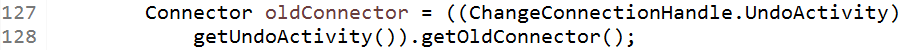
\includegraphics[width=\linewidth]{multipleLine/pic3-1}
%\caption{Alternating line number example.}
%  \label{fig:pic3-1}
%\end{figure}

%\begin{figure}[H]
%\centering
%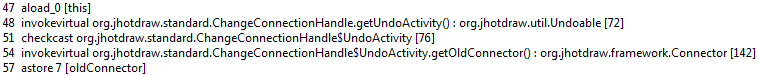
\includegraphics[width=\linewidth]{multipleLine/pic3-2}
%\caption{Bytecode to \figref{pic3-1}.}
%  \label{fig:pic3-2}
%\end{figure}

%\begin{figure}[H]
%\centering
%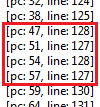
\includegraphics[width=0.3\linewidth]{multipleLine/pic3-3}
%\caption{Line number table/interval \figref{pic3-1}.}
%  \label{fig:pic3-3}
%\end{figure}

Special about this example is that the multiple line interval does not start with the smaller line number and end with the bigger one, apart from that it is alternated stored in the line number attribute.

\renewcommand\lstlistingname{Code}
\begin{Java}[caption={Nested interval example.}, label={code:2-1}, firstnumber=149]
for (int i = 0; i < ColorMap.size(); i++)
	choice.addItem(
		new ChangeAttributeCommand(
			ColorMap.name(i),
			attribute,
			ColorMap.color(i),
			this
		)
	);
\end{Java}

\renewcommand\lstlistingname{Bytecode}
\begin{JVMIS}[caption={Bytecode to \coderef{2-1}.}, label={code:2-2}, breaklines=true]
 8  iconst_0
 9  istore_3 [i]
10  goto 37
13  aload_2 [choice]
14  new org.jhotdraw.standard.ChangeAttributeCommand [213]
17  dup
18  iload_3 [i]
19  invokestatic org.jhotdraw.util.ColorMap.name(int) : java.lang.String [246]
22  aload_1 [attribute]
23  iload_3 [i]
24  invokestatic org.jhotdraw.util.ColorMap.color(int) : java.awt.Color [252]
27  aload_0 [this]
28  invokespecial org.jhotdraw.standard.ChangeAttributeCommand(java.lang.String, org.jhotdraw.framework.FigureAttributeConstant, java.lang.Object, org.jhotdraw.framework.DrawingEditor) [222]
31  invokevirtual org.jhotdraw.util.CommandChoice.addItem(org.jhotdraw.util.Command) : void [225]
34  iinc 3 1 [i]
37  iload_3 [i]
38  invokestatic org.jhotdraw.util.ColorMap.size() : int [256]
41  if_icmplt 13
\end{JVMIS}

\begin{JVMIS}[caption={Line number table/interval to \coderef{2-1}.}, label={code:2-3}, breaklines=true]
[pc: 8, line: 149]
[pc: 13, line: 150]
[pc: 14, line: 151]
[pc: 18, line: 152]
[pc: 22, line: 153]
[pc: 23, line: 154]
[pc: 27, line: 155]
[pc: 28, line: 151]
[pc: 31, line: 150]
[pc: 34, line: 149]
\end{JVMIS}

%\begin{figure}[H]
%\centering
%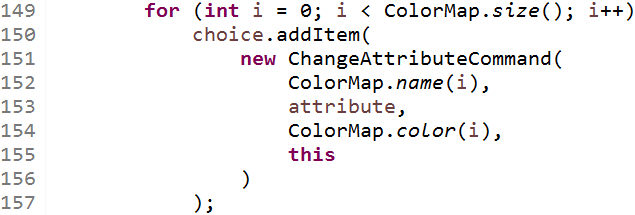
\includegraphics[width=\linewidth]{multipleLine/pic2-1}
%\caption{Nested interval example.}
%  \label{fig:pic2-1}
%\end{figure}

%\begin{figure}[H]
%\centering
%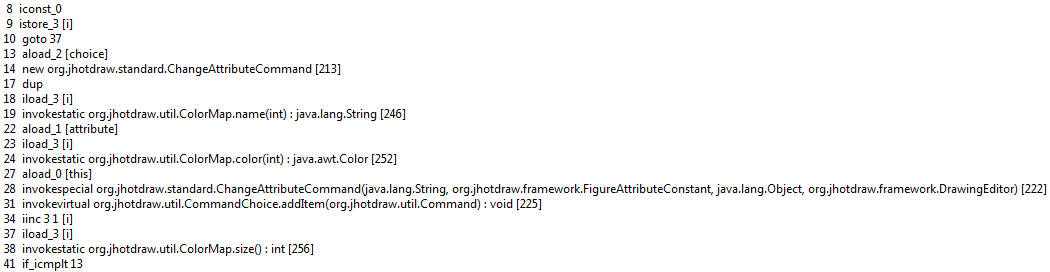
\includegraphics[width=\linewidth]{multipleLine/pic2-2}
%\caption{Bytecode to \figref{pic2-1}.}
%  \label{fig:pic2-2}
%\end{figure}

%\begin{figure}[H]
%\centering
%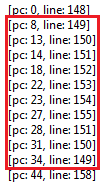
\includegraphics[width=0.3\linewidth]{multipleLine/pic2-3}
%\caption{Line number table/interval to \figref{pic2-1}.}
%  \label{fig:pic2-3}
%\end{figure}

Neither in bytecode nor in line number attribute we can extract the exact interval of method invocations. Generally, we cannot distinguish if the interval represents a method invocation or a loop. Another interesting thing is that in the figure multiple corresponding pcs are included.
\lt{change to scntactic example}
\renewcommand\lstlistingname{Code}
\begin{Java}[caption={Incomplete interval example.}, label={code:5-1}, firstnumber=22]
fooTestSupporter
	.bla(getObject(),
		staticMethod(o),
		fooTestSupporter2.bla2(null,
			o));
\end{Java}

\renewcommand\lstlistingname{Bytecode}
\begin{JVMIS}[caption={Bytecode to \coderef{5-1}.}, label={code:5-2}, breaklines=true]
18  aload_1 [fooTestSupporter]
19  invokestatic isFieldOrLocalVariableNullExample.testMethodCall.FooTest.getObject() : java.lang.Object [26]
22  aload_3 [o]
23  invokestatic isFieldOrLocalVariableNullExample.testMethodCall.FooTest.staticMethod(java.lang.Object) : java.lang.Object [30]
26  aload_2 [fooTestSupporter2]
27  aconst_null
28  aload_3 [o]
29  invokevirtual isFieldOrLocalVariableNullExample.testMethodCall.FooTestSupporter.bla2(java.lang.Object, java.lang.Object) : java.lang.Object [34]
32  invokevirtual isFieldOrLocalVariableNullExample.testMethodCall.FooTestSupporter.bla(java.lang.Object, java.lang.Object, java.lang.Object) : void [38]
\end{JVMIS}

\begin{JVMIS}[caption={Line number table/interval to \coderef{5-1}.}, label={code:5-3}, breaklines=true]
[pc: 18, line: 22]
[pc: 19, line: 23]
[pc: 22, line: 24]
[pc: 26, line: 25]
[pc: 28, line: 26]
[pc: 29, line: 25]
[pc: 32, line: 23]
\end{JVMIS}


%\begin{figure}[H]
%\centering
%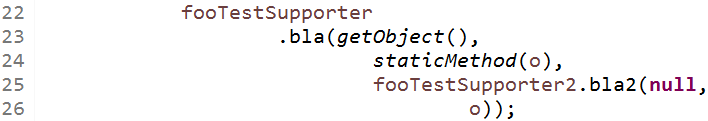
\includegraphics[width=\linewidth]{multipleLine/pic5-1}
%\caption{Incomplete interval example.}
%  \label{fig:pic5-1}
%\end{figure}

%\begin{figure}[H]
%\centering
%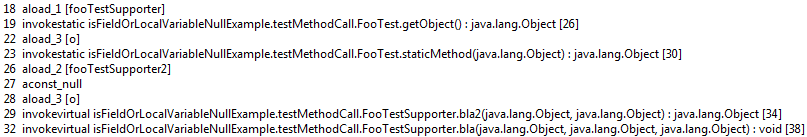
\includegraphics[width=\linewidth]{multipleLine/pic5-2}
%\caption{Bytecode to \figref{pic5-1}.}
%  \label{fig:pic5-2}
%\end{figure}

%\begin{figure}[H]
%\centering
%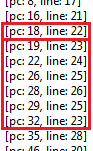
\includegraphics[width=0.3\linewidth]{multipleLine/pic5-3}
%\caption{Line number table/interval to \figref{pic5-1}.}
%  \label{fig:pic5-3}
%\end{figure}

By using the algorithm we only get the interval from pc 19-32, but actually pc 18 also belongs to the interval. That the missing pc is missing will be detected in step 4\&5 when traversing back the ArrayList by the number of parameters. If it is not a static method invocation and there is not enough possible \mrs stored in that ArrayList to traverse back, the missing pc is added in retrospect.

\renewcommand\lstlistingname{Pseudocode}
\begin{Java}[caption={Multiple line interval algorithm.}, label={alg:multipleLineAlg}]
i = index in line number attribute which contains the invoke.* opcode

if (lineNrAttribute[j>i] <= lineNrAttribute[i]) {

	if (isAlternating(i,j))
		return getAlternatingInterval(i, j);

	// non-alternating
	b = j which has the smallest line number after j;
	a = corresponding index to b; // index<k which has the same line number as b||k
	return getNonAlternatingInterval(a, b);

} else if (lineNrAttribute[j<i] == lineNrAttribute[i]) {

		b = i;
		a = j;
		return getInterval(a, b);

}
\end{Java}

This pseudocode will give a very rough idea how the invocation interval can be read out. The detailed implementation can be seen in the classes \code{MultipleLineManager}\footnote{\label{package2}In package \emph{ch.unibe.scg.nullSpy.instrumentator.controller.methodInvocation}.} and \code{MethodInvocationAnalyzer}\textsuperscript{\ref{package2}}.

\subsection{Obtaining Variable Data Difficulties - Fields}
\label{subsec:variableDifficulties}
We previously mentioned that NullSpy first collects data about fields and we met some difficulties regarding this. By using the method \code{loopBody()} from class \code{Javassist.expt.ExprEditor} (\subsecref{field}) for gathering information caused those troubles because it loops through the GIVEN \code{methodInfo} which contains the bytecode sequence of a method. Even after finding a field assignment and adding some additional bytecode to it, the method still iterates through the unchanged \code{methodInfo} it got as parameter without the additional bytecode. Getting the right start-pc of a field assignment is not a straight forward process as it may seem.

After entered extra instructions the method \code{loopBody()} iterates onwards until it finds a key which indicates an access to a field. Normally, Javassist provides a method with which the start-pc of the field access can be find out easily, but in our case not due to bytecode alternation. This method returns the start-pc of the field as if there was no changes, however it actually has to return a bigger start-pc than it does. The start-pc is needed to distinguish in what category the field has to be assigned to (\subsecref{field}).

To find the right start-pc of the field assignment, we compare the start-pc returned by a method of Javassist with the \code{afterStorePc} of the previously found field assignment. Every time an assignment is found we store it as a reference for the next assignment to obtain the right data. Even for the store-pc of an assignment (\textit{``put.*"} the last found field is essential. If there is more interest how those pcs are obtained, please see the class \code{FieldAnalyzer}\footnote{In package \emph{ch.unibe.scg.nullSpy.instrumentator.controller}.}.

\subsection{Bytecode Adaptation Difficulties}
\label{subsec:bytecodeAdaptationDifficulties}
The reason why we decided to use Javassist for our NullSpy project is because the thought of only using the source-level API \figref{bytecodeModificationLevels} to implement everything. It would have been much easier to only operate at source-level instead of learning how to read bytecode or extract data from it or enter extra code into it, yet at the end we still had to do everything at bytecode-level.

One big problem encountered while inserting the test method between an assignment and a closing bracket \code{\}}. We tried to insert additional code as shown in \figref{insertionCodeExample} by specifying the exact line number where it should be entered in source code. Unfortunately Javassist first checks the specified line whether it contains some code (only symbols excluded). If there is no code at that line it computes the next line that contains some and inserts the test method right before it. Please visualize a situation where for example a local variable is created/instantiated at the end of a \code{if-body}. In this situation Javassist adds the extra code right before the next code line which is outside the existing scope of the local variable.

\renewcommand\lstlistingname{Code}
\begin{Java}[caption={Bytecode adaptation example.}, label={code:bytecodeAdaptationExample_1}]
Object fontName;
if (fName.startsWith("A")) {
	fontName = new Arial();
} else {
	fontName = new Calibri();
}
\end{Java}

\begin{Java}[caption={Wrong Adaptation to \coderef{bytecodeAdaptationExample_1}.}, label={code:bytecodeAdaptionExample_2}]
Object fontName;
if (fName.startsWith("A")) {
	fontName = new Arial();
 } else {
	--<inserted code which takes ``fontName'' as parameter>--
	fontName = new Calibri();
}
\end{Java}


That is why changed the way to insert the test method at bytecode-level. Like this we first have to build up the bytecode sequence and then enter it before a specific pc. Please take a look at the class \code{ByteCodeAdapter}\footnote{In package \emph{ch.unibe.scg.nullSpy.instrumentator.controller}.} how the bytecode sequence is created.

There are of course many other small problems during the implementation of NullSpy but these mentioned are the most troublesome ones.

\section{Limitations}
\label{sec:limitations}
During the implementation of NullSpy we had to change the concept few times due to limitations or an overhead that could have grown immense.

Our first idea of how NullSpy could track the \npes is to gather information about variable assignment, which is the case now, and also inject another test method right before each method invocations. In small projects this way could have worked fine but in larger projects which could contain hundreds of classes with a lot of method invocations the execution time would be strongly influenced.

Being able to collect data about variables we still are not able to avoid injecting bytecode even it affects the runtime. Related to this issue a limitation about Javassist is mentioned before namely inserting bytecode right before a closing bracket (\subsecref{bytecodeAdaptationDifficulties}). Because of this it highly depends on the location where additional code should be inserted whether using the source-level API is possible or not. \ugh{Avoiding checking all the location where something new should be added it is more secure to do this on bytecode-level.}\lt{ändern} But in cases like entering something at the beginning or at the end of a method body the source-level is just fine.

Another limitation of Javassist to mention is that it does not provide anything to get information about \mrs. It only allows one to extract information about local variables, fields and method invocations itself. The programming language Java also does not provide any information about the \mr, since the exception object or the stack trace element only contains the class, file, method name and the line number. Nonetheless making possible to gather data about them the algorithm discussed before (see \algref{methodReceiverAlg}) fulfills the missing task.

The last limitation we want to discuss here is that unfortunately NullSpy is not capable to track the root of \npes that are originated in a null which was returned of a method call or in an element of a collection. Why those situations are not supported in NullSpy is because of the impossibility way to store them, e.g. imagine a nested ArrayList or a HashMap and a never ending return value of method invocations. So we lack something tangible to compare with each other, get a hit and read the location out of the hit (\secref{futureWork}).

\chapter{Validation}
\label{ch:validation}
This chapter will provide some numbers to compare the execution time each project takes, the original and the instrumented one. To get the numbers we instrumented the example project JHotDraw.

\section{JHotDraw}
\label{sec:jhotdraw}
{JHotDraw\footnote{\protect\url{http://www.jhotdraw.org/}}} also served to check whether the logic of the bytecode manipulation behind NullSpy is working as desired. JHotDraw is an open-source Java GUI framework for technical and structured Graphics. It is big enough to get reliable numbers and it provides many different cases we had to take care of in NullSpy. Also thanks to Nevena Milojkovi\'{c} and her experience with the combination Javassist and JHotDraw we as well decided to test NullSpy on it.

\section{Execution Time Difference}
\label{sec:execTimeDiff}
How did we get the numbers? First of all, of course another executable jar file of the modified project has to be created. The steps to it are followings: load project, modify project, store modified project, build project that creates an executable jar file of the original project and one of the modified one. We then simulate the terminal with a Java class to run each jar thirty times and calculate the average. The next table lists each execution time and the average:

\begin{table}[H]
\centering
\begin{tabular}{ l | S[table-format=1.3] | S[table-format=1.3]|}
\cline{2-3}	  &\textbf{Original project} & \textbf{Modified project}\\ \cline{2-3}
	1	& 7.223	& 7.442	\\ \cline{2-3}
	2	& 7.427	& 7.738	\\ \cline{2-3}
	3	& 7.171	& 7.893	\\ \cline{2-3}
	4	& 7.035	& 7.379	\\ \cline{2-3}
	5	& 7.488	& 7.458	\\ \cline{2-3}
	6	& 7.194	& 7.691	\\ \cline{2-3}
	7	& 6.849	& 7.472	\\ \cline{2-3}
	8	& 7.286	& 8.068	\\ \cline{2-3}
	9	& 7.083	& 7.519	\\ \cline{2-3}
	10 & 7.27	& 7.55	\\ \cline{2-3}
	11 & 7.16	& 7.177 \\ \cline{2-3}
	12 & 7.161  & 7.55	\\ \cline{2-3}
	13 & 7.225	& 7.223	\\ \cline{2-3}
	14 & 7.037	& 7.316	\\ \cline{2-3}
	15 & 7.067	& 7.54	\\ \cline{2-3}
	16 & 6.975	& 7.77	\\ \cline{2-3}
	17 & 7.287	& 7.117	\\ \cline{2-3}
	18 & 7.52	  & 7.488	\\ \cline{2-3}
	19 & 7.303	& 7.35	\\ \cline{2-3}
	20 & 6.942	& 7.307	\\ \cline{2-3}
	21 & 7.147	& 7.535	\\ \cline{2-3}
	22 & 7.222	& 7.644	\\ \cline{2-3}
	23 & 7.145	& 7.32	\\ \cline{2-3}
	24 & 7.334	& 8.187	\\ \cline{2-3}
	25 & 7.364	&7.488	\\ \cline{2-3}
	26 & 7.269	&7.942	\\ \cline{2-3}
	27 & 7.441	&7.943	\\ \cline{2-3}
	28 & 7.223	&7.467	\\ \cline{2-3}
	29 & 6.912	&7.647	\\ \cline{2-3}
	30 & 7.363	&7.784	\\ \cline{2-3}
	\cline{2-3}
	\end{tabular}
	\caption{Execution time.}
	\label{tab:executionTime}
\end{table}

\begin{table}[H]
	\centering
	\begin{tabular}{ | S[table-format=1.4] | S[table-format=1.6] |}
		\hline
		\textbf{Original project} & \textbf{Modified project}\\ \hline
		7.2041	&	7.566834 \\
		\hline
	\end{tabular}
	\caption{Average time.}
	\label{tab:averageTime}
\end{table}

The runtime of the modified project takes 0.362734s longer than the original one, this means after adding additional code to the project results in approximately \textbf{5\%} overhead. This small overhead is quite negligible. But this numbers have to be interpreted with caution because the overhead is only measured on JHotDraw.

\chapter {Conclusion and Future Work}
\label{ch:conclusionFutureWork}
Now we have come so far to retrospect (step back and have a critical loot at) the entire project for summarizing what goals we have achieved so far and for proposing further aims that could be completed in the future. In a small section we also want to talk about the gained experience during the whole project.

\section{NullSpy}
\label{sec:nullSpy}
Happily, we could say here that we successfully managed to meet the main purpose we have set at the beginning of the project. NullSpy is now capable to tracking the \npes to its root and provide the user with more information about its origin without spending much time on finding it. The most important steps which lead to the success of NullSpy are listed below:

\begin{enumerate}
\item Extract and gather information about all \mrs because method invocations on these causes \npes. To achieve this, we developed an algorithm (\algref{methodReceiverAlg}) with the function of finding \mrs and extracting data from it by only doing static bytecode analysis. The information about it is then stored as an external csv file. It is needed for a comparison in in a later step.

\item Again collecting data, but this time about variable assignments namely local variables and fields. Here next to the static bytecode analysis additional instructions are inserted to the class files to check right after the assignment if the variable is assigned to the special value \code{null}. If this is the case everything about the variable is stored in a HashMap which serves for a comparison too. It is stored in a HashMap because if a variable is assigned to another object than null, it will be deleted from the HashMap.

\item NullSpy does only handle the uncaught \npe which means we can wrap up the \code{main()} method with a catch block. In this catch block the class name and the line number where the \npe occurred is extracted from the stack trace. This information is passed to a method in which the parameter helps to find the guilty \mr. With the hit the exact location where that variable was set to null can be derived from the HashMap.

\item All the additional needed classes are added to the project after it is modified and stored in a folder the user has chosen. Being able to run the modified project of course a jar file is created. In our case JHotDraw already provides a \textit{build.xml} which we had to alternate a little bit.
\end{enumerate}

During the implementation we were encountered with many difficulties. Some of those we were able to solve and some not unfortunately. Those unsolved ones could be proposed as goals of future work. The next section will list some of them.

\section{Future Work}
\label{sec:futureWork}
\subsection{Support unsupported \mrs and variable assignments}
As mentioned in (\secref{limitations}), if the cause of a \npe lies in an element of a collection or in an object that is returned by a method invocation, it cannot be tracked to its assignment location. Come up with a way to extract and store information could be a future aim. Of course gathering information about the \mrs has to be improved too.

\subsection{Track \npe root for all projects}
As now our goal in this project was tracking null assignments of JHotDraw. First of all, we had to make sure that building JHotDraw works properly with the additional classes. To fulfil this task manual changes on the build.xml was necessary. If this can be done automatically by NullSpy it would be much better.

Next to this we only looked at the assignment and \mr types which appear in JHotDraw itself. There could be other types that are not covered in NullSpy depending on projects. In case NullSpy is used on projects that contain not supported issues improving it to cover them can be added to the toDo list.

\subsection{Plug-in for Eclipse}
Last target for future work to mention here is transform NullSpy into an Eclipse compatible plug-in project. After integrated it with Eclipse the null tracking can be started without any expenses on how to manipulate the build.xml if there is one or even bother to create an executable jar file out of it.

For now, we can only think of these future work that could improve NullSpy to give it more value.

\section{Personal Experience}
At the beginning, after reading the description of the project I had no clue how to approach its goal at all. Since this is my first big project on my own but with help from two experienced research assistants I learned a lot, especially in the matter of programming.

As the project is all about manipulating class files, here with Javassist, we first had to learn how bytecode is constructed and get familiar with Javassist. Luckily there is a very good tutorial that teaches one how to use it. This class library however does not cover everything we needed. Thanks to this we had to deal with the lack extensively and learned quite a lot about working on bytecode-level.

Next to getting familiar with bytecode we also had to invent algorithms like that of extracting \mrs from the bytecode or that of getting the pc-interval of a \mr. It was quite interesting to invent those as these are the first ones that fulfill more complex tasks.

Debugging: It is not as easy as it seems. Sometimes it took hours to find the cause of a small bug, and after fixing it another occurs. The reason why it took that long to debug is because along with checking whether the logic of our code was right we also had to find the right bytecode position to ensure the implementation does what it is created for.

Coding beautifully the way so that it will not smell was another challenge due to lack of experience. Sometimes I tended to put everything in one class instead of abiding by the single responsibility principle. Therefore, refactoring the whole project multiple times was necessarily which also took some time. Best before starting to code is to clearly thinking through what is needed, how the structure should look like and what kind of responsibility each class of the project should take for gaining time for other things.

We also came in contact with the building XML file and the jar file. Concerning the XML file, we gained experience by learning a new language by modifying it that it also creates a jar file out of the modified project.



%END Doc
%-------------------------------------------------------

\bibliography{scg}
\bibliographystyle{plain}

\begin{appendices}

% A N L E I T U N G  Z U  W I S S E N S C H A F T L I C H E N  A R B E I T E N
% % % % % % % % % % % % % % % % % % % % % % % % % % % % % % % % % % % % % % % %
\chapter {Anleitung zu wissenschaftlichen Arbeiten}
NullSpy is a program which helps Java developers to find the root of \npes by providing an additional link next to the common stack trace. The key idea behind NullSpy is to help developers to save time fixing bugs which are caused by \npe. Of course this approach tries to provide this service by keeping the overhead to a minimum. To demonstrate how NullSpy works, this chapter serves as a small tutorial that takes JHotDraw as the testing project to show the feature of NullSpy.

\section{Installation}
\label{sec:installation}
For this tutorial JHotDraw is needed. In order to download it, visit the following site and download ``JHotDraw6.0 beta 1'' (version we worked with during the implementation of NullSpy):\\
\href{http://www.jhotdraw.org}{www.jhotdraw.org}\\
Unpack the archive and store it to a location of your choice. To be able to run JHotDraw additional libraries are used, that are not included in JHotDraw itself. Following libraries are to be downloaded:\\
``batik-all-1.7'': \href{http://www.java2s.com/Code/Jar/b/Downloadbatikall17jar.htm}{www.java2s.com/Code/Jar/b/Downloadbatikall17jar}\\
``jdo'': \href{http://www.java2s.com/Code/Jar/j/Downloadjdojar.htm}{www.java2s.com/Code/Jar/j/Downloadjdojar}\\
Again unpack those archives and store them in a lib folder in your JHodDraw project.

Running the tests of JHotdraw with the commando line the location of libraries ``hamcrest'' and ``junit'' are needed, which are normally also downloaded when the programming environment Eclipse\footnote{Can be downloaded here: \href{https://eclipse.org/downloads/}{www.eclipse.org/downloads}} is downloaded.

\chapter{Bytecode combinations of \mrs}
\label{cha:bytecodeCombinations}
In \subsecref{methodReceiver} we discussed about extracting all possible combinations of \mrs which are embedded in the outermost interval. We developed a system for identifying them by using the following list shown in \listref{methodReceiverTemplate}.

\begin{figure}[H]
\renewcommand\figurename{List}
	\begin{boxedminipage}{\textwidth}
		\begin{itemize}
		\itemsep8pt
		\item local variable
		\begin{itemize}
			\item aload													y
			\item aload.getfield 								y	
			\item aload.getfield.getfield...		y	(if fields are public)
			\item aload.getstatic								n	(aload = ref, getstatic = arg)
			\item aload.aload\_0									n	(aload = ref, this.getfield etc = args
			\item aload.aload										n	(aload = ref, aload = arg)
			\item aload.new											n	(aload = ref, new = arg)
		\end{itemize}
   
		\item non-static field
		\begin{itemize}
			\item aload\_0												y	(aload\_0 = ref for private method)
			\item aload\_0.getfield							y	
			\item aload\_0.getfield.getfield. ..	y	(if getfields are public fields)
			\item aload\_0.this									n	(aload\_0 = ref, this... = arg)
			\item aload\_0.getfield.getstatic		n (!exist)
			\item aload\_0.getstatic							n	(aload\_0 = ref, getstatic = arg)
			\item aload\_0.aload									n	(aload\_0 = ref, aload = arg)
			\item aload\_0.new										n	(aload\_0 = ref, new = arg)
		\end{itemize}

		\item static field
		\begin{itemize}
			\item getstatic											n	(ignore, because getinvoke)
			\item getstatic.aload								n
			\item getstatic.aload\_0							n
			\item getstatic.new									n
			\item getstatic.getstatic						n (!exist)
			\item getstatic.getfield						y
			\item getstatic.getfield.getfield.	y	(getfields are public field)
		\end{itemize}
   \end{itemize}
	\end{boxedminipage}
	\caption{\Mr template.}
	\label{list:methodReceiverTemplate}
\end{figure}

While we iterate through the invocation pc-interval and run into the opcode \eg \textit{``aload.*''} we check what comes after this opcode. If \textit{getfield} is the following opcode, we know that the bytecode represents a field access of a local variable or of the current analyzed class depending on which local variable slot the opcode \textit{``aload.*''} refers to. Next again, we check the next opcode after \textit{getfield} and so on until the following opcode does not fit into the allowed pattern of the template. As long as the checked opcode fits into our template, we consider them as one possible \mr.

If the following opcode after the first \textit{``aload.*} is another \textit{``aload.*} we can be sure that they are two separate \mr candidate because two local variables does not have any relationship with each other. Even if the first opcode is a \textit{aload\_0}.

With this system we iterate through the outermost invocation pc-interval and split it into candiate \mr pc-intervals.

\end{appendices}

\clearpage
\thispagestyle{empty}
\null\vfill
\begin{center}
''Ich erkl\"are hiermit, dass ich diese Arbeit selbstst\"andig verfasst und  keine  anderen  als  die  angegebenen  Quellen  benutzt  habe.
Alle Stellen, die w\"ortlich oder sinngem\"ass aus Quellen entnommen  wurden,  habe  ich  als  solche  gekennzeichnet.  Mir  ist  bekannt,  dass  andernfalls  der  Senat  gem\"ass  Artikel 36  Absatz 1 Buchstabe
r  des  Gesetzes  vom  5. September 1996  \"uber  die  Universit\"at zum Entzug des auf  Grund dieser Arbeit verliehenen Titels berechtigt ist.“
\end{center}
\vfill
\clearpage

\end{document}
